\chapter{Single fiber simulations} \label{chap:three}

We perform three numerical experiments that involve two substrates and one fiber of a reasonable length ($n=96$) in order to determine the equilibrium configurations of the substrate-fiber system. In the first experiment we study a single fiber attached to the bottom substrate. We start with a fiber perpendicular to the substrate and allow it to relax. We observe that in the absence of an external load there are two generic possibilities, either that the fiber remains free standing or that it adheres to the substrate. We consider a particle of a fiber adhered to a substrate if there exists a substrate particle such that the distance between both particles is approximately equal to that of the vdW equilibrium. A criterion for adhesion between two vectors describing particles of the system $\textbf{a}$ and $\textbf{b}$ is thus defined, 
\begin{equation} \label{eqn:criterion}
	$\|\textbf{a} - \textbf{b}\| \lessapprox \sigma$
\end{equation}
Further a fiber is adhered to a substrate if at least one particle of the fiber is adhered to that substrate. In our simulations we used the following heuristic for particle adhesion, 
\begin{eqnarray} \label{eqn:adhesion}
	A(\textbf{a}, \textbf{b}) &=& \left\{ 
		\begin{array}{ll}
			0, & \|\textbf{a} - \textbf{b}\| \leq 1.1 \sigma + 10^{-6}\\
			1, & \mbox{otherwise}
		\end{array}
		\right.  \\
	A_+ &=& \sum_{j=1}^{m} \sum_{i=1}^{n} \left[ 1 - \prod_{k=1}^{n_+} A(\textbf{r}_i^{(j)},\textbf{r}_k^{(+)}) \right] \label{eqn:adhesion:top} \\ 
	A_- &=& \sum_{j=1}^{m} \sum_{i=1}^{n} \left[ 1 - \prod_{k=1}^{n_-} A(\textbf{r}_i^{(j)},\textbf{r}_k^{(-)}) \right]. \label{eqn:adhesion:bottom}
\end{eqnarray}
Here the equilibrium distance, $\sigma$, between two particles is relaxed by $10\%$ and an additional factor of $10^{-6}$ to take into account simulation precision. A fiber particle is counted as adhered only once, regardless of how many substrate particles it is adhered to.

The second experiment includes the top substrate with an associated load applied to it. Starting from the same initial configuration as the first experiment we observe if and how the fiber is compressed by the top substrate. This experiment is motivated by the subsequent detachment experiment. Here we are interested in finding a load applied to the top substrate such that the equilibrium configuration has all fiber particles adhered to the bottom substrate (and thus to the top substrate).

The third experiment we take the target equilibrium configuration obtained in the second experiment and reverse the direction of the load on the top substrate. We are interested in finding the loads that will break adhesion of the top substrate with the fiber. The adhesion heuristics (\ref{eqn:adhesion:top}) and (\ref{eqn:adhesion:bottom}) are used as a method of categorizing different equilibrium configurations for varying parameters.

\section{The free standing fiber experiment}

The model has two kinds of pairwise bonds between particles---strong and weak. Strong bonds cannot be broken and include the extensible springs between adjacent particles on a fiber and the attachment bond to the bottom substrate. Weak bonds on the other hand can be broken and correspond to vdW interaction between various particles in the system. We considered particles weakly bonded if they satisfy the criterion (\ref{eqn:criterion). We already defined adhesion as a weak bond between a substrate and fiber particles. Now in addition we define crystallization as another weak bond between any two non-adjacent fiber particles satisfying the same criterion. Generally our simulations show that if any two fiber particles crystallize then other fiber particles will crystallize as well.

	\begin{figure}[ht!]
		\begin{center}
			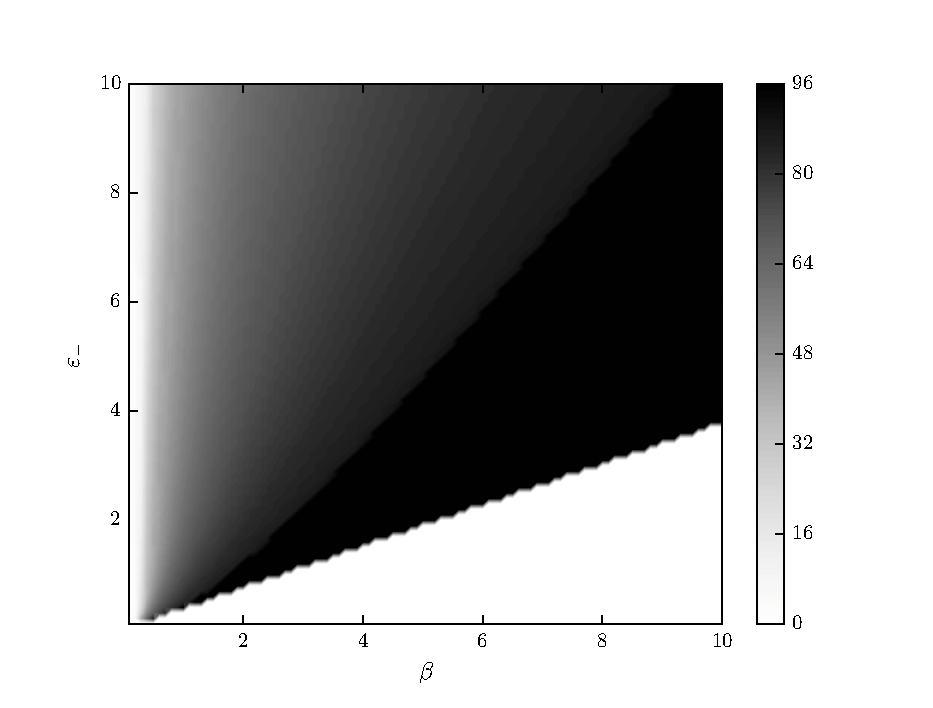
\includegraphics{./fig/ch3/fs/grid.eps}
		\end{center}		
		\caption{Plot of torsional spring strength, $\beta$, by bottom substrate vdW strength, $\eps_-$, colored by adhered (fiber) particle count to the bottom substrate. There are three distinct regions that categorize the behavior of a fiber: the black region of flattened fibers, the white region of standing or slanted fibers, and the grey sub-regions.
		\label{fig:fs}}
	\end{figure}

We say a fiber is \textit{flattened} if every particle of the fiber is adhered to the bottom substrate. If the parameters of the system are such that a fiber is flattened in the free standing experiment then it will be flattened under any values of the external load in the compression experiment. We determine the parametric ranges for which the fiber becomes flattened. We conjecture that here the critical role is played by the torsional spring and vdW interaction between the fiber and bottom substrate. Although, inter-fiber vdW interactions may also play a role we have not vary them here.

	%% Fallen Figures
	\begin{figure*}[h!]
		\centering
		\begin{subfigure}{.5\textwidth}
			\centering
			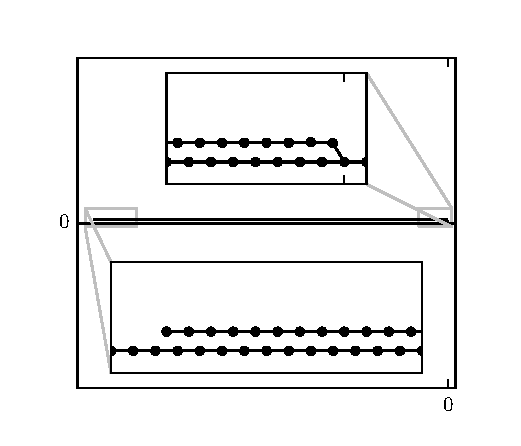
\includegraphics{./fig/ch3/fs/b5_eb3.eps}
			\caption{$\beta=5$ and $\eps_-=3$.\label{subfig:lazy}}
		\end{subfigure}%
		~
		\begin{subfigure}{.5\textwidth}
			\centering
			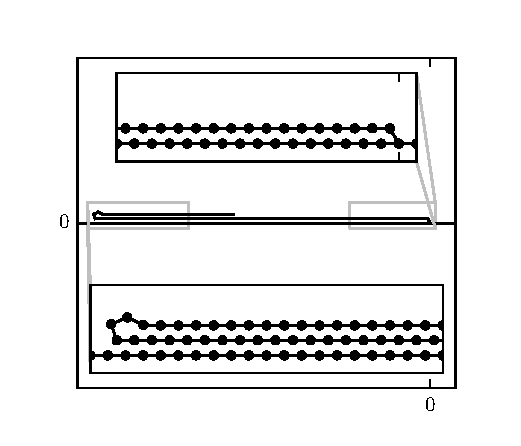
\includegraphics{./fig/ch3/fs/b2_eb6.eps}
			\caption{$\beta=2$ and $\eps_-=6$.\label{subfig:lazy_loop}}
		\end{subfigure}

		\begin{subfigure}{.5\textwidth}
			\centering
			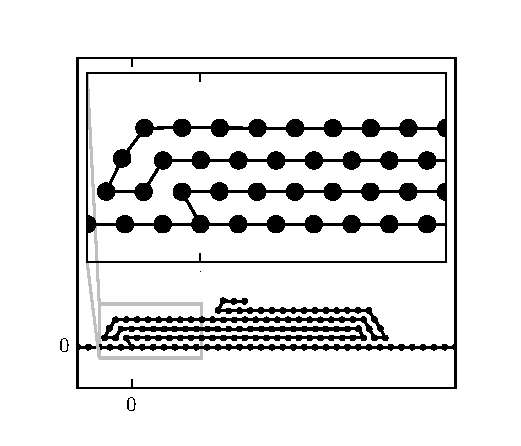
\includegraphics{./fig/ch3/fs/b0.5_eb10.eps}
			\caption{$\beta=0.5$ and $\eps_-=10$.\label{subfig:lazy_many_loops}}
		\end{subfigure}		
		\caption{The black region of Figure~\ref{fig:fs} consists strictly of (a) flattened fibers. (b) Configurations that contain a single kink are located in the grey region near the black region. (c) Configurations with additional kinks are located farther away.\label{fig:lazy}}	
	\end{figure*}

We vary $\beta$ and $\eps_-$ as shown in Figure~\ref{fig:fs} (colored according to the value of $A_-$ in (\ref{eqn:adhesion:bottom})). If the fiber buckles there are necessarily fiber particles that can not be adhered. It must then be the case that the black region corresponds to flattened configurations only (see Figure~\ref{subfig:lazy} for example). 

	%% Erect Figures
	\begin{figure*}[t!]
		\centering
		\begin{subfigure}{.5\textwidth}
			\centering
			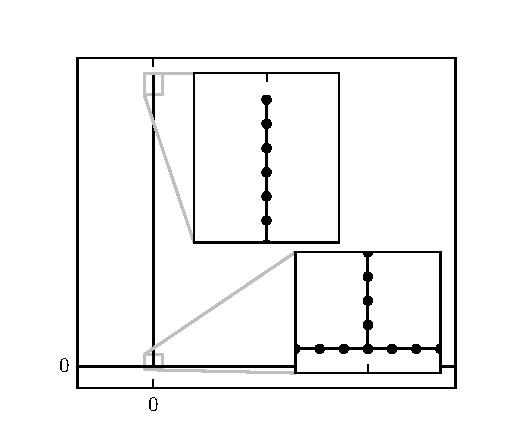
\includegraphics{./fig/ch3/fs/b10_eb1.eps}
			\caption{$\beta=10$ and $\eps_-=1$.\label{subfig:erect}}
		\end{subfigure}%
		~
		\begin{subfigure}{.5\textwidth}
			\centering
			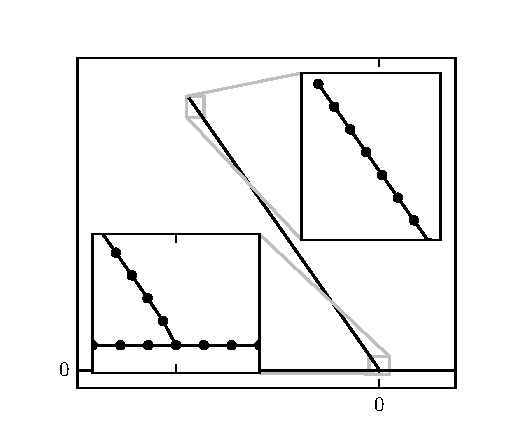
\includegraphics{./fig/ch3/fs/b10_eb3.eps}
			\caption{$\beta=10$ and $\eps_-=3$.\label{subfig:leaning}}
		\end{subfigure}
		\caption{The white region of Figure~\ref{fig:fs} consists strictly of standing fibers. A standing fiber does not need to be (a) orthogonal to the bottom substrate, but can be (b) slanted and straight or curved.\label{fig:alert}}
	\end{figure*}

	%% Crystalized Figures
	\begin{figure*}[h!]
		\centering
		\begin{subfigure}{.5\textwidth}
			\centering
			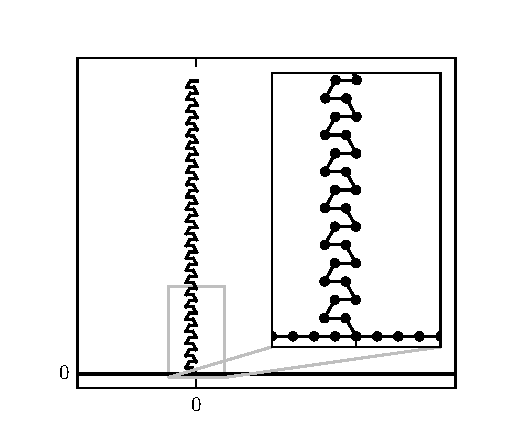
\includegraphics{./fig/ch3/fs/b0.1_eb0.5.eps}
			\caption{$\beta=0.1$ and $\eps_-=0.5$.\label{subfig:hex_chain}}
		\end{subfigure}%
		~
		\begin{subfigure}{.5\textwidth}
			\centering
			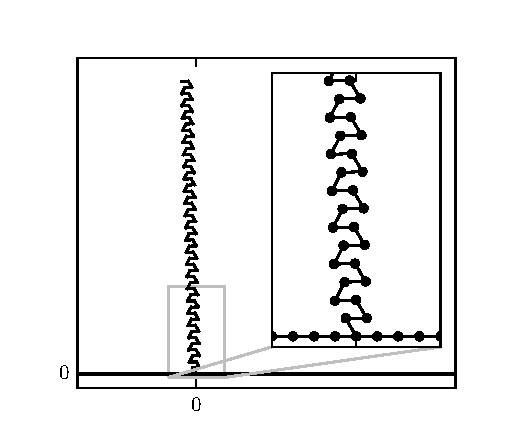
\includegraphics{./fig/ch3/fs/b0.1_eb3.eps}
			\caption{$\beta=0.1$ and $\eps_-=3$.\label{subfig:leaning_hex_chain}}
		\end{subfigure}

		\begin{subfigure}{.5\textwidth}
			\centering
			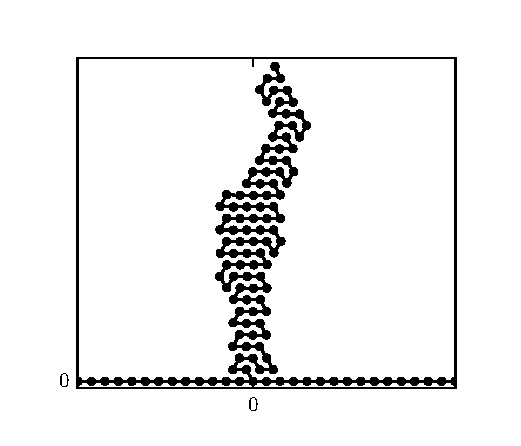
\includegraphics{./fig/ch3/fs/b0.2_eb3.eps}
			\caption{$\beta=0.2$ and $\eps_-=3$.\label{subfig:crystal1}}
		\end{subfigure}%
		~
		\begin{subfigure}{.5\textwidth}
			\centering
			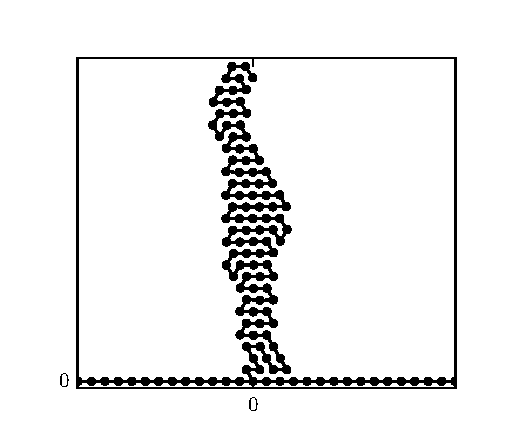
\includegraphics{./fig/ch3/fs/b0.2_eb9.eps}
			\caption{$\beta=0.2$ and $\eps_-=9$.\label{subfig:crystal2}}
		\end{subfigure}	
		\caption{Small $\beta$ of Figure~\ref{fig:fs} corresponds to fibers that crystallize with themself. Note the specific kind of crystallization of (a) and (b) as a pseudo-hexagonal chain configuration of the particles. Kinds of crystallization can be similar as with (c) and (d) but sutbly different.\label{fig:crystal}}	
	\end{figure*}

The white region of the plot consists of configurations were the fiber is either orthogonal to the bottom substrate, slanted but straight, or curved. In fact, we conjecture that a significant bend can only happen at the root, that all other particles are negligibly bent, and that if the root particle adheres to the bottom substrate then all particles will. Consider that the root particle of the fiber is nearest to the bottom substrate and will experience the strongest vdW interaction with the bottom substrate relative to any other fiber particle. Indeed, if the vdW interaction causes the root particle torsional spring to bend but not buckle, then the force applied to the immediate next particle will be significantly smaller creating a negligible bend, and so on. If the vdW interaction is strong enough to cause the root particle to adhere to the bottom substrate then the torsional spring and the vdW interaction will move the next particle into an adhered state, and then the next, and so on. Observe the linear relationship between $\beta$ and $\eps_-$ at the dividing line between the white and black region in Figure~\ref{fig:fs} which matches our conjecture. With sufficiently large $\beta$ relative to $\eps_-$ the fiber is not slanted (see Figure~\ref{subfig:erect}), and as $\beta$ decreases and $\eps_-$ increases, staying in the white region of Figure~\ref{fig:fs}, the fiber becomes more slanted (see Figure~\ref{subfig:leaning}).

The grey subregions of the plot are more complex and corresponds to buckling of fiber particles other than the root or fiber crystallization. Near the black region as $\eps_-$ is increased there is a gradual change from one buckle to two and so on. It appears that the particle at which buckles occur happen closer to the root with increased $\eps_-$. The linear relationship between $\beta$ and $\eps_-$ is qualitatively present between not only the white and black region, but the black and grey, and different grey subregions. However, as $\beta$ decreases the slope increases. This trend hints that with smaller $\beta$ the fiber is more likely to crystallize. Crystallization for small $\beta$ is difficult to categorize with our adhesion heuristic, but Figure~\ref{fig:crystal} presents example crystallization equilibrium configurations to help with our intuition. Most notably there are configurations where the fiber can be said to be still ``standing'' as if the inter-fiber vdW interaction has replaced torsional springs as a method of fiber stiffness (see Figure~\ref{subfig:hex_chain} and Figure~\ref{subfig:leaning_hex_chain}).

\section{Compression}

	\begin{table}[th]
		\rowcolors{1}{}{lightgray}
		\centering
		\caption{Reference parameters for compression.\label{table:compression_reference}}
		\begin{tabular}{lcrclcr}
			$m$ & = & 1 & \hspace{1in} & $\ell_-$ & = & 1 \\
			$n$ & = & 96 & & $\ell_+$ & = & 1 \\
			$n_+$ & = & 400 & & $\ell$ & = & 1 \\
			$n_-$ & = & 200 & & $\gamma$ & = & 100 \\
			$x^{(-)}$ & = & -100 & & $\beta$ & = & 10 \\
			$y^{(-)}$ & = & 0 & & $\eps_-$ & = & 1 \\
			$x^{(+)}$ & = & -200 & & $\eps_+$ & = & 1 \\
			$y^{(+)}$ & = & 110 & & $\eps$ & = & 1 \\
			$\delta$ & = & 0 & & $\sigma$ & = & 1
		\end{tabular}
	\end{table}
For the compression experiment a fiber is initially standing (see Figure~\ref{subfig:erect}). The primary focus is equilibrium configurations of the fiber under varying loads from the top substrate. Initially the top substrate is sufficiently far away from every particle on the fiber to prevent any vdW interaction, and because of this only loads with some nonzero positive vertical component are considered. A set of reference parameters in Table~\ref{table:compression_reference} are used in every case unless values are explicitly stated otherwise.

\subsection{Reference parameters}

	\begin{figure}[t]
		\begin{center}
			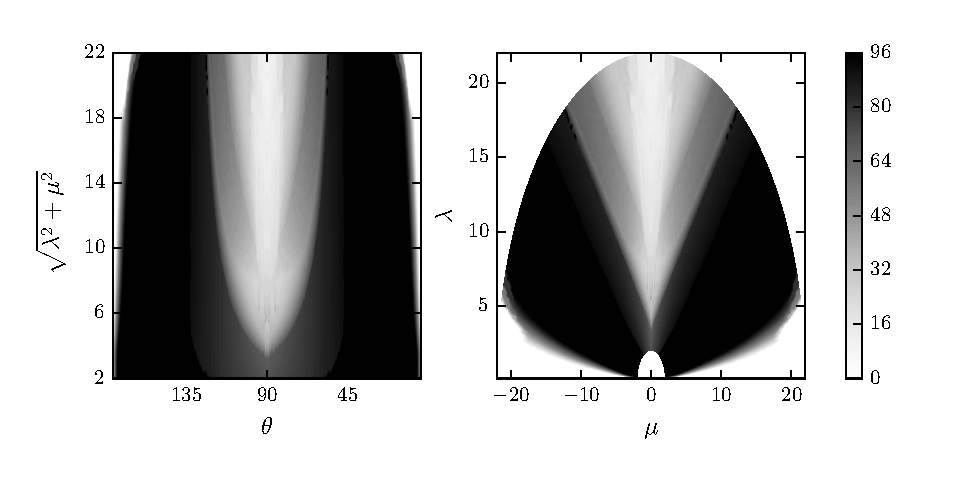
\includegraphics{./fig/ch3/push/ref/grid.eps}
		\end{center}		
		\caption{Plot of vertical component of load applied to the top substrate, $\lambda$, by the horizontal component, $\mu$, colored by adhered (fiber) particle count to the top substrate on the right. On the left is the same plot represented instead by the angle of the load by the load's magnitude colored in the same way. The black region consists of fibers that are in the \textit{flattened} configuration. There are obvious qualitative delineations of the plot by color but the categorization of the associated fiber configuration is not trivial.
		\label{fig:push:ref}}
	\end{figure}

Figure~\ref{fig:push:ref} plots the horizontal component of the load applied to the top substrate by its vertical component colored by the adhesion heuristic (\ref{eqn:adhesion:top}). Analysis of contour plots of this kind will be the main focus of the results presented for the compression experiment. As with the free standing experiment, the black region of the plot corresponds to a flattened configuration (see Figure~\ref{subfig:flattened}). Aside from the black region there are other qualitative features of the plot: a white region, three distinct grey regions with sufficiently large magnitude of the load, small dark patches between two of those grey regions, and small grey patches in the white region for small magnitude of the load. We will explore the different regions of the plot through example.

For the darkest grey region we select $\lambda=14$ and $\mu=10.5$ as seen in Figure~\ref{subfig:flat_loop}. The configuration has one buckling point or \textit{kink}. A \textit{kink} is a buckle in a fiber that consists of relatively few particles and has sharp interior angles between bonds. This is in contrast to what we consider a \textit{bend} in a fiber which consists of potentially many particles with small interior angles between bonds. For the darkest grey region we conjecture that as the angle of the load on the top substrate, $\theta$, is increased from $45$\textdegree\ the particle at which the kink in the fiber occurs will change to one further up the chain, thus causing less particles to be adhered.

	\begin{figure*}[h!]
		\centering
		\begin{subfigure}{.5\textwidth}
			\centering
			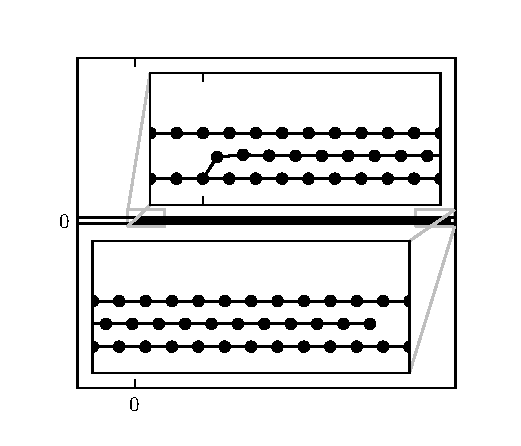
\includegraphics{./fig/ch3/push/ref/l5_m10.eps}
			\caption{$\lambda=5$ and $\mu=10$.\label{subfig:flattened}}
		\end{subfigure}%
		~
		\begin{subfigure}{.5\textwidth}
			\centering
			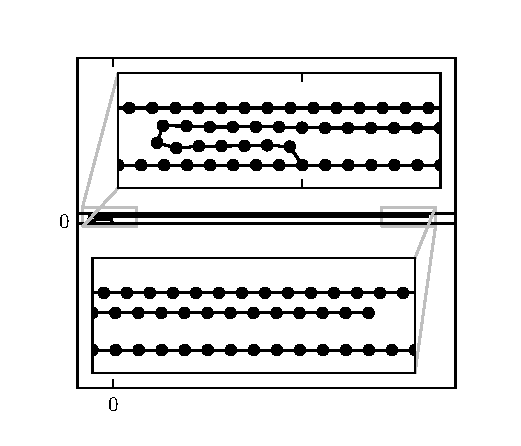
\includegraphics{./fig/ch3/push/ref/l14_m10.5.eps}
			\caption{$\lambda=14$ and $\mu=10.5$. \label{subfig:flat_loop}}
		\end{subfigure}

		\begin{subfigure}{.5\textwidth}
			\centering
			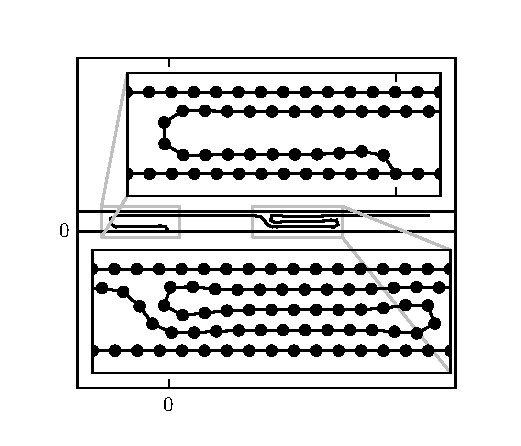
\includegraphics{./fig/ch3/push/ref/l15.5_m6.eps}
			\caption{$\lambda=15.5$ and $\mu=6$.\label{subfig:lonely_pancake}}
		\end{subfigure}%
		~
		\begin{subfigure}{.5\textwidth}
			\centering
			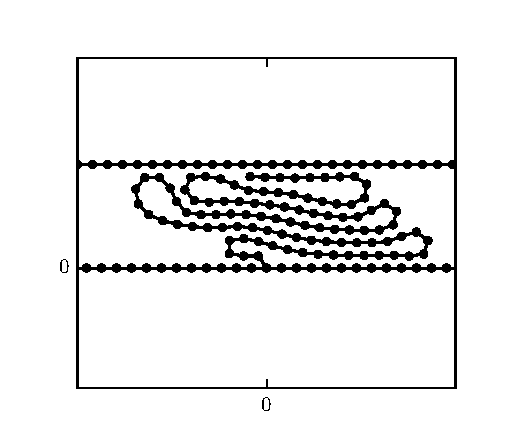
\includegraphics{./fig/ch3/push/ref/l19_m0.5.eps}
			\caption{$\lambda=19$ and $\mu=0.5$.\label{subfig:crushed}}
		\end{subfigure}
		\caption{Fiber configurations using the reference parameters in Table~\ref{table:compression_reference} with varying load. A contour plot of the adhered particle count is shown in Figure~\ref{fig:push:ref}. The black region of contour plot corresponds to (a) flattened fibers. They white region corresponds to configurations with (d) many folds. The grey region is complex and has different configurations two of which are shown in (b) and (c).\label{fig:ref_normal}}
	\end{figure*}

	\begin{figure*}[th!]
		\centering
		\begin{subfigure}{.5\textwidth}
			\centering
			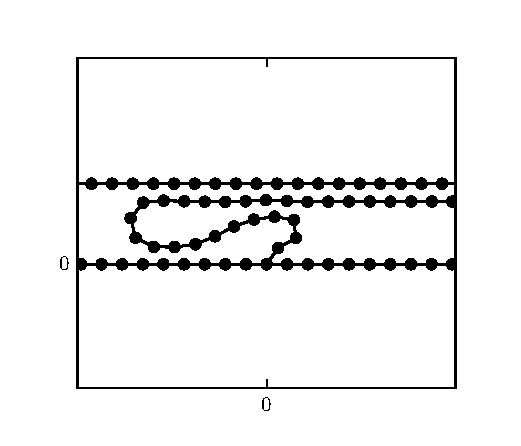
\includegraphics{./fig/ch3/push/ref/l17_m11.eps}
			\caption{$\lambda=17$ and $\mu=11$.\label{subfig:tight_loop}}
		\end{subfigure}%
		~
		\begin{subfigure}{.5\textwidth}
			\centering
			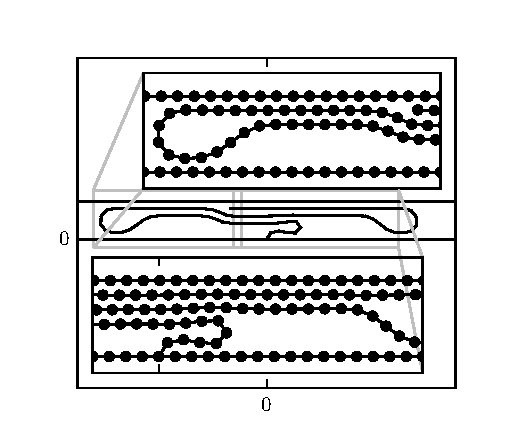
\includegraphics{./fig/ch3/push/ref/l5.9_m0.1.eps}
			\caption{$\lambda=5.9$ and $\mu=0.1$.\label{subfig:tight_hairpin}}
		\end{subfigure}
		\caption{Fiber configurations using the reference parameters in Table~\ref{table:compression_reference} with varying load. There are two locations in the contour plot of Figure~\ref{fig:push:ref} that are curious. There are patches of black between the whiter region and grey region of the plot (shown in (a)), and there are small grey pathces near the bottom of the white region (shown in (b)).\label{fig:ref_special}}
	\end{figure*}

The next darkest grey region does not have any observable difference between it and the following grey region. Configurations shown in Figure~\ref{subfig:lonely_pancake} or configurations very similar to it were observed in both grey regions of the plot. Although the pattern associated with the adhesion heuristic is not obvious it appears that with stronger vertical component, $\lambda$, the fiber contains more buckles.

Figure~\ref{subfig:crushed} describes the kinds of configurations that are found in the white region. The fiber is ``crushed'' underneath the load of the top substrate causing several kinks and bends. The mechanism in which some particles are able to adhere to the top substrate while others are kept crystallized underneath the folds of the fiber itself is beyond the descriptive power of the adhesion heuristic. However, with variance in the white region in mind, equilibrium configurations are still likely to have the same ``crushed'' geometry.

Two special regions of the plot are the black patches between the darker two grey regions and the grey patches near $\theta=90$\textdegree\ with small magnitude. Figure~\ref{subfig:tight_loop} is an example of a configuration in the black patch region and Figure~\ref{subfig:tight_hairpin} is an example of a configuration in the grey patch region. Both configurations have bends in contrast to other configurations with kinks and similar loads.

	\begin{figure}[t]
		\begin{center}
			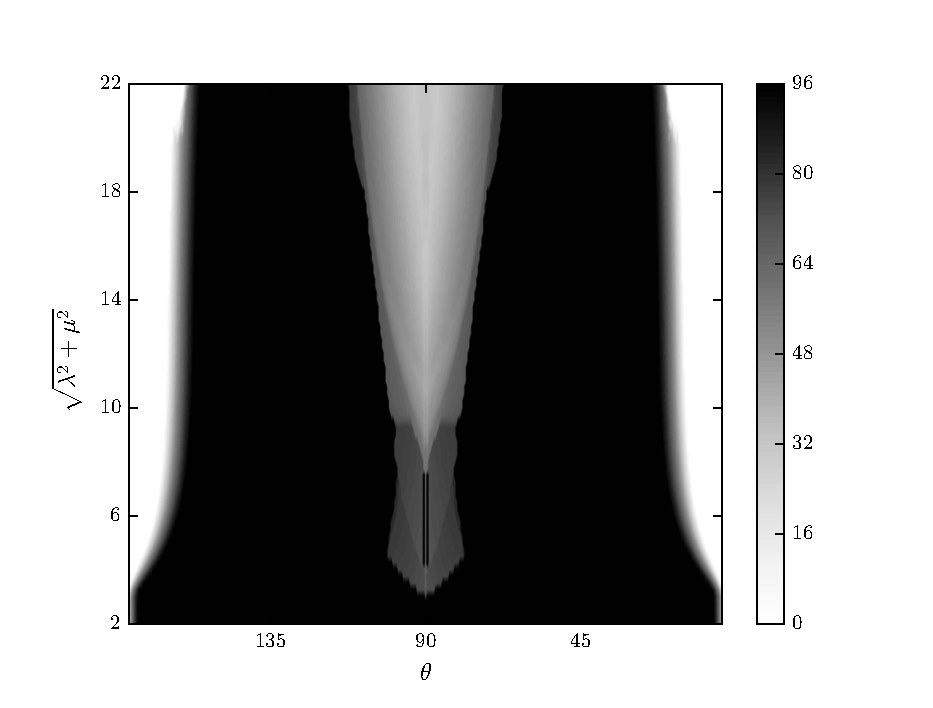
\includegraphics{./fig/ch3/push/b100/grid.eps}
		\end{center}		
		\caption{Plots of adhesive modes of a fiber under compression as in Figure~\ref{fig:push:ref}. Torsional spring strength is increased from reference parameters, $\beta=100$.
		\label{fig:push:b100}}
	\end{figure}	
	
	\begin{figure}[t]
		\begin{center}
			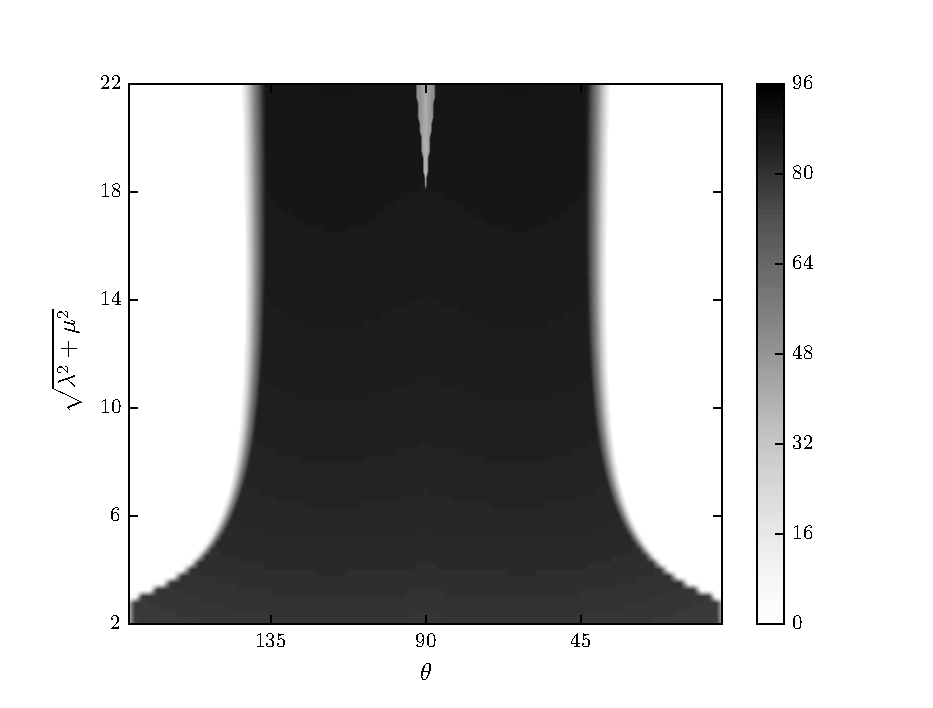
\includegraphics{./fig/ch3/push/b1000/grid.eps}
		\end{center}	
		\caption{Plots of adhesive modes of a fiber under compression as in Figure~\ref{fig:push:ref}. Torsional spring strength is increased from reference parameters, $\beta=1000$. The grey gradient from the top of the plot to the bottom immediately means that there is no strictly flattened fiber configuration.
		\label{fig:push:b1000}}
	\end{figure}
	
	\begin{figure*}
		\centering
		\begin{subfigure}{.5\textwidth}
			\centering
			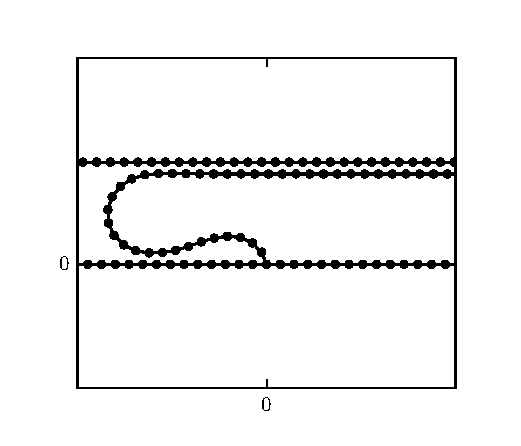
\includegraphics{./fig/ch3/push/b100/l4.6_m0.65.eps}
			\caption{$\lambda=4.6$ and $\mu=0.65$.\label{subfig:short_loop}}
		\end{subfigure}%
		~
		\begin{subfigure}{.5\textwidth}
			\centering
			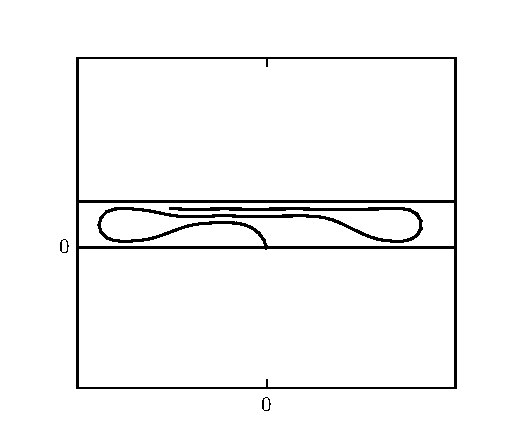
\includegraphics{./fig/ch3/push/b100/l19_m0.eps}
			\caption{$\lambda=19$ and $\mu=0$.\label{subfig:hairpin}}
		\end{subfigure}

		\begin{subfigure}{.5\textwidth}
			\centering
			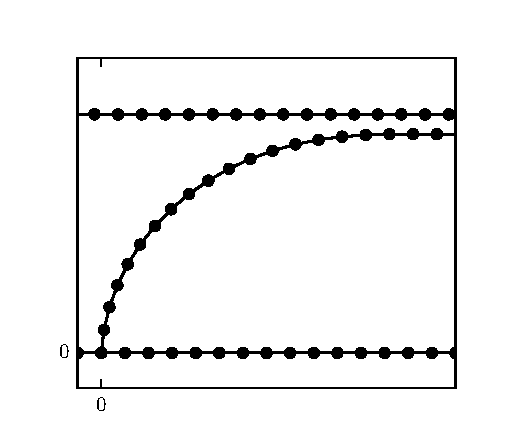
\includegraphics{./fig/ch3/push/b1000/l3_m2.eps}
			\caption{$\lambda=3$ and $\mu=2$.\label{subfig:curved}}
		\end{subfigure}%
		~	
		\begin{subfigure}{.5\textwidth}
			\centering
			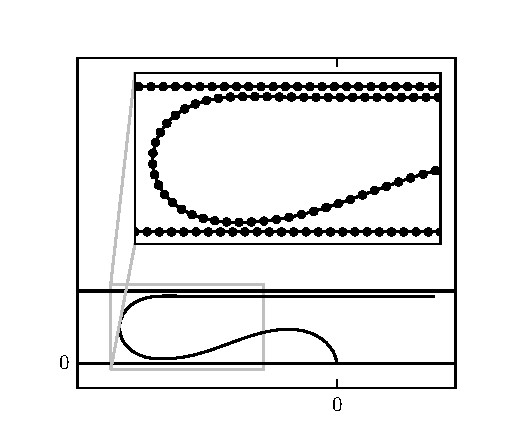
\includegraphics{./fig/ch3/push/b1000/l20_m0.eps}
			\caption{$\lambda=20$ and $\mu=0$.\label{subfig:long_loop}}
		\end{subfigure}	
		\caption{Fiber configurations using the reference parameters in Table~\ref{table:compression_reference}. Configurations (a) and (b) modify the reference paramters torsional spring string, $\beta=100$. Configurations (c) and (d) modify the same paramter, $\beta=1000$. From all configurations we note that an increase in $\beta$ correspondes to bends consisting of many particles instead of kinks consisting of few particles.\label{fig:bending_fiber}}	
	\end{figure*}

\subsection{Varying $\beta$}

The strength of the torsional spring strength, $\beta$, is important to a fiber moving to a flattened configuration or a standing configuration. For the reference parameters in Table~\ref{table:compression_reference} $\beta$ is strong enough to stand freely. However, decreasing the reference value of $\beta$ by an order of magnitude would make it too small for the fiber to stand freely. Because of this we focus on increasing $\beta$.

Increasing $\beta$ by an order of magnitude such that $\beta=100$ significantly alters the picture from before. Shown in Figure~\ref{fig:push:b100} the black region of the plot is larger and grey and white regions are narrow and have different shape. The difference in configurations for each region has to do with how many fiber particles are part of a bend or if there is more than one bend. We present two examples: Figure~\ref{subfig:short_loop} corresponds to the black line inside the darker grey region, and Figure~\ref{subfig:hairpin} corresponds to $\theta=90$\textdegree\ with large magnitude.

The grey region of the contour plot is a similar configuration in Figure~\ref{subfig:short_loop} with the exception that more of the fiber is folded underneath itself causing a wave-like curve. The white regions also are similar to the example given in Figure~\ref{subfig:hairpin}. There is variability in the adhesion heuristic but it is because of small variation in number of particles that are part of the bends of the fiber. This is the same idea shown in Figure~\ref{fig:push:ref} were slightly lighter portions of grey regions were because of configurations with a few particles being before instead of after the kink(s).

Increasing $\beta$ by another order of magnitude, $\beta=1000$, again significantly alters the picture. Figure~\ref{fig:push:b1000} shows the contour plot with this modification. Most notable is the loss of a black region, and a significantly smaller white region. The gradient of the grey region is represented in it's entirety with Figure~\ref{subfig:curved}. Any configuration in the grey region is only a fiber with a gradual bend from the root to the first adhered particle on the top substrate. This configuration is novel to $\beta=1000$ and likely impossible for $\beta=100,10$. The white region in contrast is similar to the same kind of configurations seen in the grey regions of $\beta=100$ with the exception of even more particles as part of the bend (see Figure~\ref{subfig:long_loop}).

	\begin{figure}[t]
		\begin{center}
			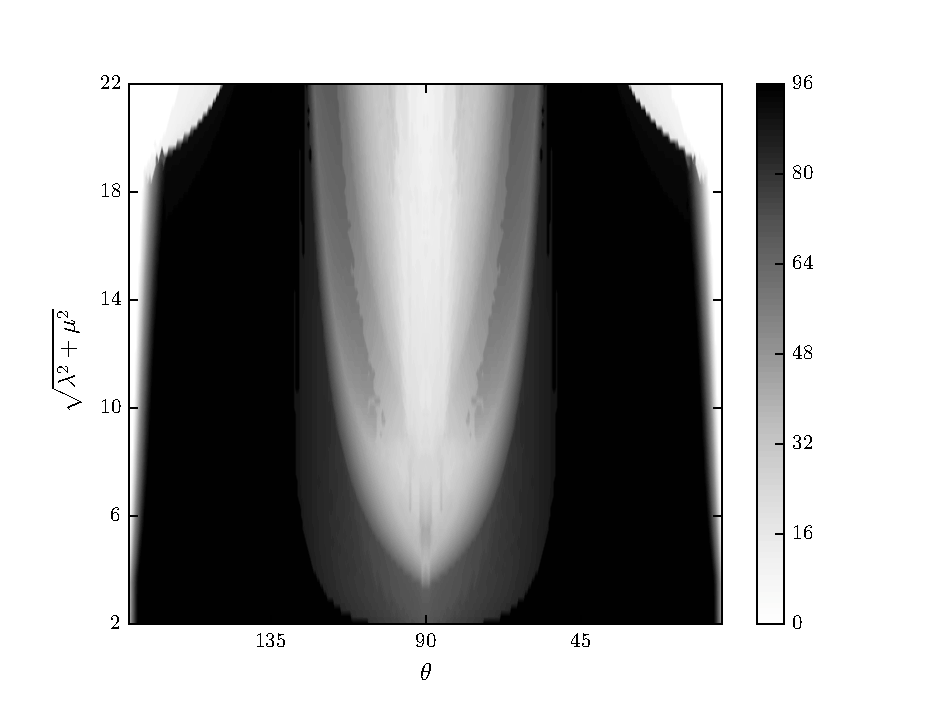
\includegraphics{./fig/ch3/push/eb0.1/grid.eps}
		\end{center}		
		\caption{Plots of adhesive modes of a fiber under compression as in Figure~\ref{fig:push:ref}. VdW interaction strength of the bottom substrate is weakened, $\eps_-=0.1$.
		\label{fig:push:eb0.1}}
	\end{figure}	

	\begin{figure}[t]
		\begin{center}
			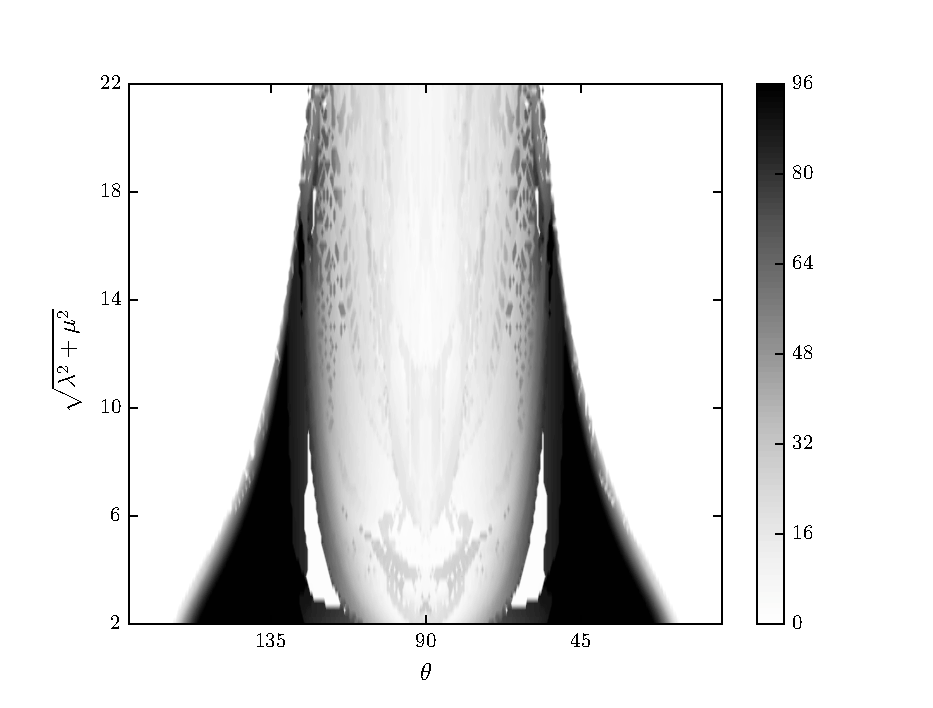
\includegraphics{./fig/ch3/push/et0.1/grid.eps}
		\end{center}		
		\caption{Plots of adhesive modes of a fiber under compression as in Figure~\ref{fig:push:ref}. VdW interaction strength of the top substrate is weakened, $\eps_+=0.1$. We note the dramatic change between this plot and Figure~\ref{fig:push:eb0.1} as they both are a weakening in vdW interaction by one order of magnitude.
		\label{fig:push:et0.1}}
	\end{figure}

	\begin{figure}[t]
		\begin{center}
			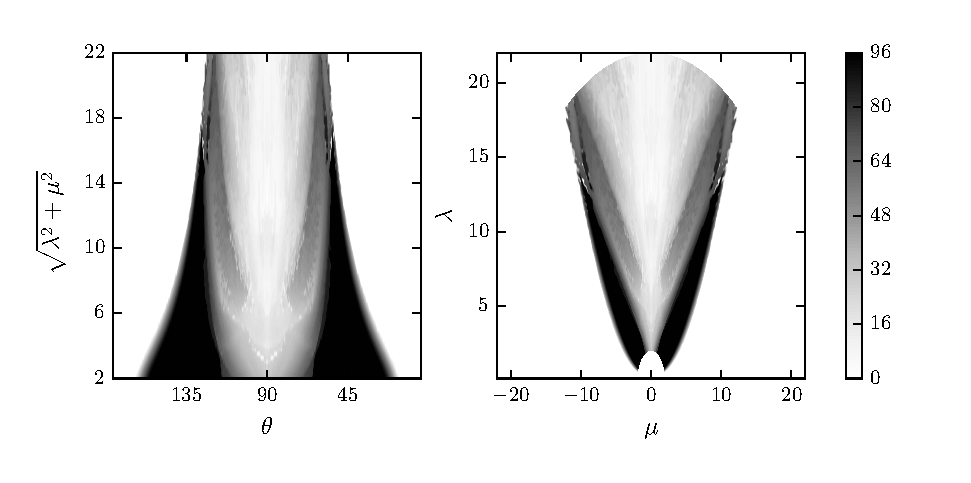
\includegraphics{./fig/ch3/push/eb0.1_et0.1/grid.eps}
		\end{center}		
		\caption{Plots of adhesive modes of a fiber under compression as in Figure~\ref{fig:push:ref}. VdW interaction strength of the top and bottom substrate is weakened, $\eps_+=0.1$ and $\eps_-=0.1$.
		\label{fig:push:eb0.1_et0.1}}
	\end{figure}	

	\begin{figure*}
		\centering
		\begin{subfigure}{.5\textwidth}
			\centering
			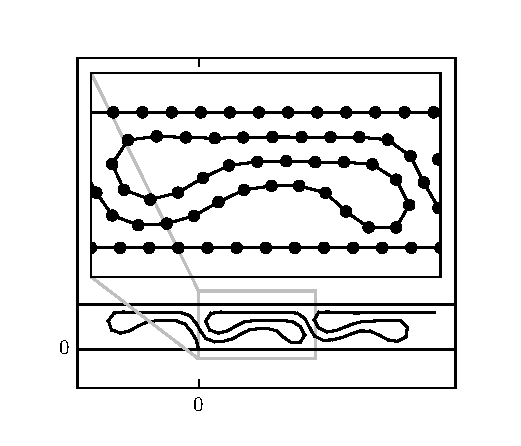
\includegraphics{./fig/ch3/push/eb0.1/l20.5_m3.5.eps}
			\caption{$\lambda=20.5$ and $\mu=3.5$.\label{subfig:multi_bridge}}
		\end{subfigure}%
		~
		\begin{subfigure}{.5\textwidth}
			\centering
			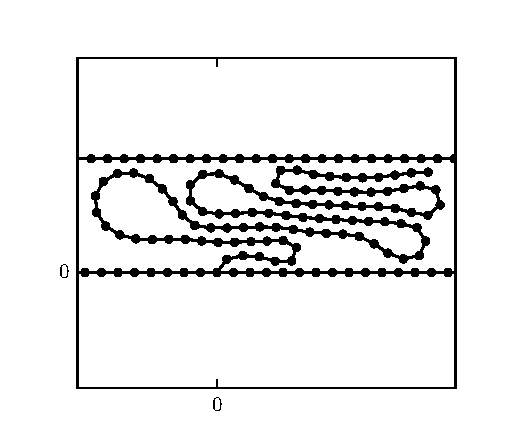
\includegraphics{./fig/ch3/push/eb0.1_et0.1/l20_m2.eps}
			\caption{$\lambda=20$ and $\mu=2$.\label{subfig:slant_crushed}}
		\end{subfigure}

		\begin{subfigure}{.5\textwidth}
			\centering
			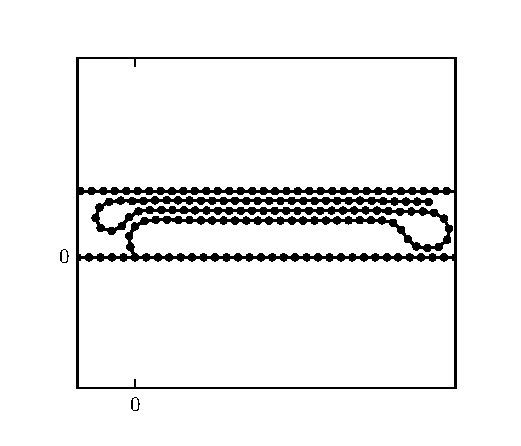
\includegraphics{./fig/ch3/push/et0.1/l4.5_m1.eps}
			\caption{$\lambda=4.5$ and $\mu=1$.\label{subfig:bridge}}
		\end{subfigure}%
		~
		\begin{subfigure}{.5\textwidth}
			\centering
			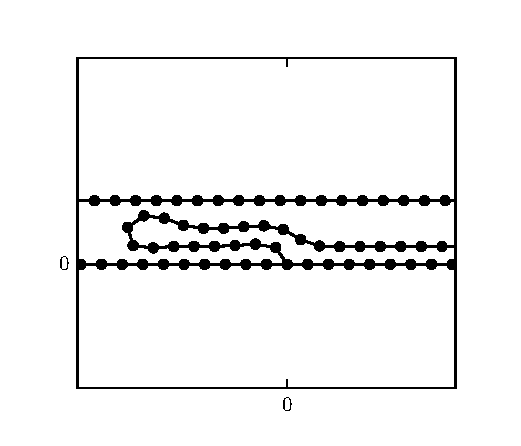
\includegraphics{./fig/ch3/push/et0.1/l6_m4.eps}
			\caption{$\lambda=6$ and $\mu=4$\label{subfig:hump}}
		\end{subfigure}	
		\caption{Fiber configurations using the reference parameters in Table~\ref{table:compression_reference}. Configuration (a) modifies the reference paramters bottom substrate vdW interaction strength, $\eps_-=0.1$. Configuration (b) modifies the reference paramters bottom and top substrate vdW interaction strength, $\eps_-=0.1$ and $\eps_+=0.1$. Configurations (c) and (d) modify the reference parameters top substrate vdW interaction strength, $\eps_+=1$.\label{fig:vdw_crushed}}	
	\end{figure*}

\subsection{Varying $\eps_-$ and $\eps_+$} \label{subsection:push:eps}

Another method of allowing a fiber to stand instead of move to a flattened configuration is to decrease the vdW interaction strengths. Namely, we are interested in decreasing the vdW interaction strengths of both substrates, first independently and then together.

As a fiber is being compressed by the top substrate, it either began the process of adhering to the bottom substrate before the top substrate was able to interact with it, or stood freely and is compressed by the top substrate. For the reference parameters the fiber will not collapse on it's on. Decreasing vdW interaction strength of the bottom substrate, $\eps_-=0.1$, is a further relaxation that emphasizes the vdW interaction with the top substrate over the vdW interaction with the bottom substrate. However, after the fiber has been compressed the bottom substrate can stiffen the fiber's configuration. Figure~\ref{fig:push:eb0.1} shows the contour plot with this modification. Although there are noticeable differences the picture is qualitatively similar to the reference parameters picture, Figure~\ref{fig:push:ref}.

In contrast, when we decrease vdW interaction strength of the top substrate, $\eps_+=0.1$, the picture becomes significantly more complex (see Figure~\ref{fig:push:et0.1}). Previously we partitioned contour plots into regions using the adhesion heuristic as a guide. However, when we decrease vdW interaction strength the complexity in configurations becomes difficult to manage. In Figure~\ref{fig:push:et0.1} we have a white region for small magnitude of the load which corresponds to a ``hump'' configuration of the fiber (see Figure~\ref{subfig:hump}). The top substrate vdW interaction strength is weaker which relaxes the constraints on the fiber both while it is being compressed and after it has been compressed. This allows for a kink to form near the root and for the fiber to completely adhere to the bottom substrate.

Decreasing vdW interaction strengths of both substrates to $0.1$ is shown in Figure~\ref{fig:push:eb0.1_et0.1}. With these modifications the primary modes of buckling involve parts of the fiber crystallizing. The grey region of the plot is similar to configurations shown in the reference parameters, specifically Figure~\ref{subfig:lonely_pancake}. The white region is also similar, consisting of ``crushed'' fiber configurations. Example configurations for decreased vdW interaction strength are shown in Figure~\ref{fig:vdw_crushed}. These examples demonstrate some of the kinds of buckling that are exhibited but large categorizations of configurations are difficult.
	
	\begin{figure}[t]
		\begin{center}
			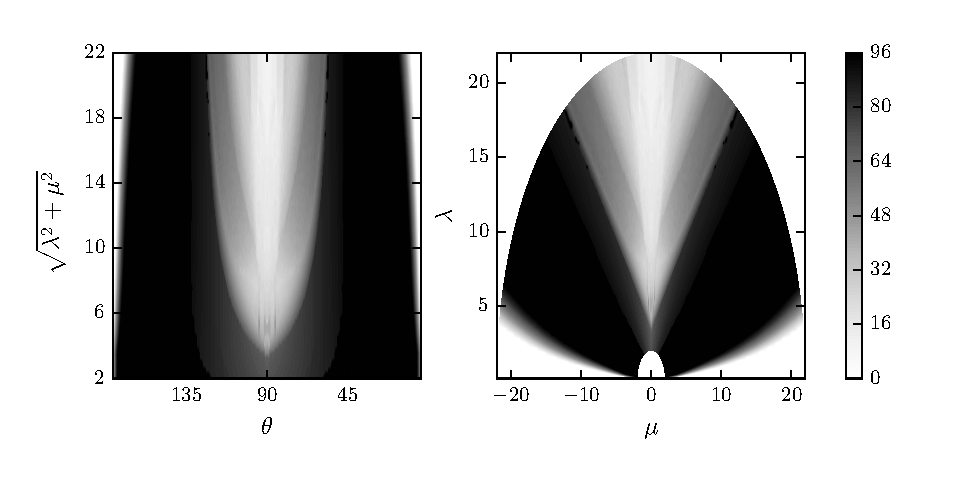
\includegraphics{./fig/ch3/push/g1000/grid.eps}
		\end{center}		
		\caption{Plots of adhesive modes of a fiber under compression as in Figure~\ref{fig:push:ref}. Extensible spring constant is increased, $\gamma=1000$.
		\label{fig:push:g1000}}
	\end{figure}	

\subsection{Varying $\gamma$}

We modify the extensible spring constant to ensure that our reference selection, $\gamma=100$, is sufficiently large to make bonds of fiber particles stiff. Figure~\ref{fig:push:g1000} for $\gamma=1000$ shows a contour plot similar to the reference plot (see Figure~\ref{fig:push:ref}). There are no qualitative differences between them which suggests that our selection of $\gamma$ is adequate.

	\begin{figure}[t]
		\begin{center}
			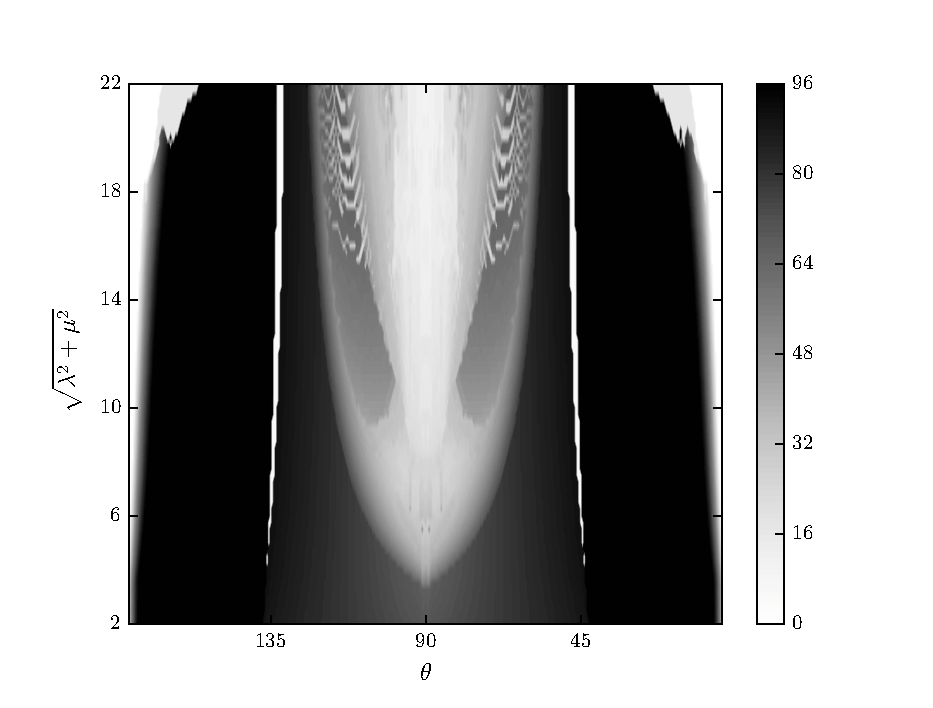
\includegraphics{./fig/ch3/push/p1/grid.eps}
		\end{center}		
		\caption{Plots of adhesive modes of a fiber under compression as in Figure~\ref{fig:push:ref}. The bottom substrate is replaced with a continuum of particles, that is the vdW interaction is integrated over the a bottom substrate of infinite length. The strength of the continuum vdW interaction is $p=1$.
		\label{fig:push:p1}}
	\end{figure}

\subsection{Bottom substrate with uniform potential} \label{section:compression:pressure}

A tangential curiosity is how the system behaves when the bottom substrate is a uniform potential instead of particle-particle potentials. We assume the bottom substrate is composed of infinitely many particles by integrating the Lennard-Jones potential. Every particle of the fiber interacts with the bottom substrate by this uniform potential instead.

Using the adhesion heuristic we see a similar picture to the reference parameters for the uniform potential (see Figure~\ref{fig:push:p1}). There are differences, notably the white region of the plot between the black and dark grey regions. This region is the same kind of ``hump'' configuration seen before in Figure~\ref{subfig:hump}. Overall, we conjecture from both plots, Figure~\ref{fig:push:ref} and Figure~\ref{fig:push:p1}, that the different potentials give the same general behavior for the equilibrium configurations of the fiber, with some exceptions. This is however a limited comparison and those exceptions are not minor.

\section{Detachment} \label{ch:detachment}

   \begin{table}[t]
      \rowcolors{1}{}{lightgray}
      \centering
      \caption{Reference parameters for the detachment experiment. \label{table:detachment_reference}}
      \begin{tabular}{lcrclcr}
         $m$ & = & 1 & \hspace{1in} & $\ell_-$ & = & 1 \\
         $n$ & = & 96 & & $\ell_+$ & = & 1 \\
         $n_+$ & = & 300 & & $\ell$ & = & 1 \\
         $n_-$ & = & 300 & & $\gamma$ & = & 100 \\
         $x^{(-)}$ & = & -150 & & $\beta$ & = & 1 \\
         $y^{(-)}$ & = & 0 & & $\eps^-$ & = & 1 \\
         $x^{(+)}$ & = & -150 & & $\eps^+$ & = & 1 \\
         $y^{(+)}$ & $\approx$ & 1.72741 & & $\eps$ & = & 1 \\
         $\delta$ & = & 0 & & $\sigma$ & = & 1
      \end{tabular}
   \end{table}

In both the free standing and compression experiments we focused on a range of values of interest and presented a contour plot of the space using a heuristic for adhesion. With the detachment experiment we can explore the parameter space more intelligently. Instead of an exhaustive approach we assume that there is a critical magnitude of the load applied to the top substrate such that it will \textit{detach} from the fiber. The top substrate is said to detach from the fiber at the point in time when no particles of the fiber are adhered to the top substrate. If there is in fact a critical magnitude of the load for a given angle of the load then we can heuristically pick a sufficiently large magnitude such that the top substrate does detach and then bisect between that value and $0$. The existence of a critical magnitude for detachment is not guaranteed and will be discussed when it is a bad assumption.

All simulations for the detachment experiment begin with the system in a flattened configuration (see Figure~\ref{subfig:flattened}). Although there are several compressed configurations from the previous experiment we focus only on the flattened configuration in this experiment.
   
   \begin{figure}[t]
      \begin{center}
         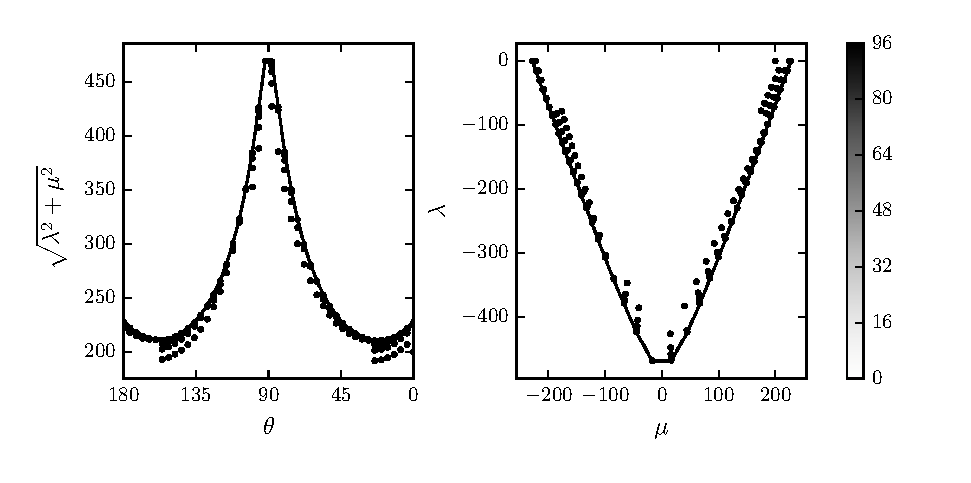
\includegraphics{./fig/ch3/pull/ref/grid.eps}
      \end{center}      
      \caption{The left is a plot of minimum critical load for the top substrate to detach from the fiber as function of the angle of the load. The right is the same plot in terms of the horizontal and vertical component of the load on the top substrate. For any given angle the critical load is only approximate, thus there are actually two lines drawn, one solid black representing the smallest detachment load, and a dashed line beneath it representing the largest adhesive load. Each circle represents a specific simulation.
      \label{fig:pull:ref}}
   \end{figure}

\subsection{Reference parameters}

As with the compression experiment we have a set of selected reference parameters in Table~\ref{table:detachment_reference}. Figure~\ref{fig:pull:ref} shows the critical magnitude for detachment of the load as a function of the angle of the load on the left, and the same line plotted via the components of the load on the right. There is a linear interpolation between every $4$th angle in the plot which makes determining extrema to high absolute accuracy difficult but we are more interested in qualitative trends anyway. Every circle of the plot is a simulation for some specific value of $\lambda$ and $\mu$, and the color of the circle is the value of the adhesion heuristic (\ref{eqn:adhesion:top}). All plots of the critical magnitude for detachment will follow these patterns.

Unlike the compression experiment, the detachment experiments do not yield as interesting equilibrium configurations. Above the critical magnitude in every case is a return to the free standing experiment with a different initial condition, and although that is interesting in it's own way the equilibrium configurations of those cases are not the focus. Thus we ignore any equilibrium configurations that happen above the critical magnitude. For the reference parameters, equilibrium configurations below the critical magnitude are all identical, they are the flattened configuration. In order to understand the picture then we turn to discussing the dynamics of the system with a detaching magnitude.

In the range $0 \leq \theta < 45$ the top substrate detaches from the fiber by sliding. The top substrate is said to ``slide'' if for a given particle on the top substrate it shifts from being adhered to one collection of fiber particles to being adhered to a different collection of fiber particles in a finite amount of time. We conjecture that the existence of a minimum in this range of $\theta$ values is because there is an optimal angle of the load to maximize the number of particles that are ``skipped'' when the top substrate slides across the fiber. As the angle of the load increases the effective horizontal displacement of the top substrate is reduced instead of improved.

   \begin{figure}[t]
      \begin{center}
         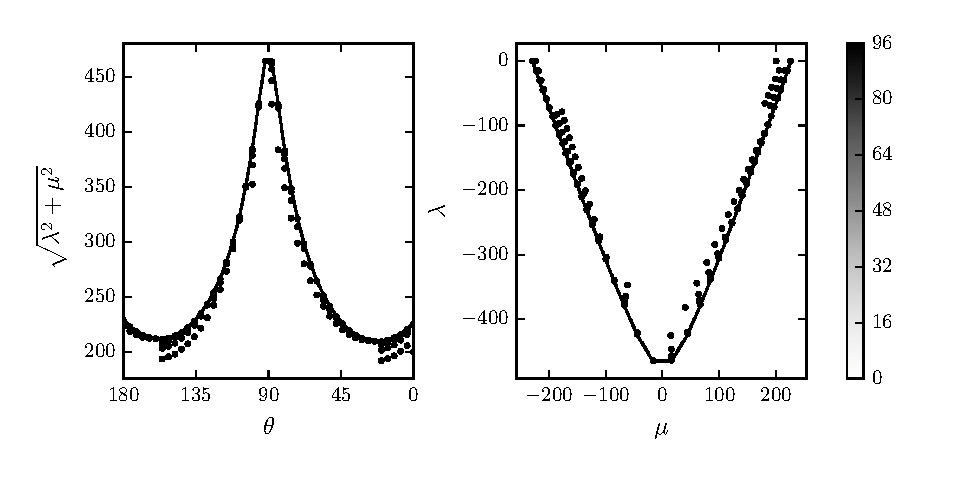
\includegraphics{./fig/ch3/pull/b10/grid.eps}
      \end{center}      
      \caption{Plot of the minimum critical magnitude for detachment as in Figure~\ref{fig:pull:ref}. The torsional spring strength is increased, $\beta=10$, from the reference parameters in Table~\ref{table:detachment_reference}.
      \label{fig:pull:b10}}
   \end{figure}

Considering the range $45 \leq \theta < 90$ the top substrate continues the sliding mode of detachment up until what is assumed to be a critical angle where the effective horizontal displacement of a single particle on the top substrate is too small to slide over a single particle of the fiber. At this critical angle the mode of detachment changes from sliding to brute force. The top substrate is said to detach from the fiber via ``brute force'' if the critical magnitude of the load must be large enough to break every vdW interaction between the fiber and the top substrate simultaneously.

The range $90 \leq \theta \leq 180$ is similar. There is a critical angle of the load such that the top substrate changes from detaching from the fiber via brute force to detaching from the fiber by sliding, and there is a minimum angle of the load such that the displacement of a given particle on the top substrate is maximized during sliding. However, the way in which sliding occurs is subtly different. There is also an observable asymmetry in the plot. One explanation is that if the top substrate pulls against the direction that the fiber has been flattened (in this case to the right) then the torsional spring energy will push a particle of the fiber up into the top substrate repelling it from the fiber making it easier to slide.

The plot on the right of Figure~\ref{fig:push:ref} tells the same story from a different perspective. With it we can see that the critical load is a linear relationship between the components of the load $\lambda$ and $\mu$ on either side of $\theta=90$\textdegree.
   
\subsection{Varying $\beta$}

   \begin{figure}[t]
      \begin{center}
         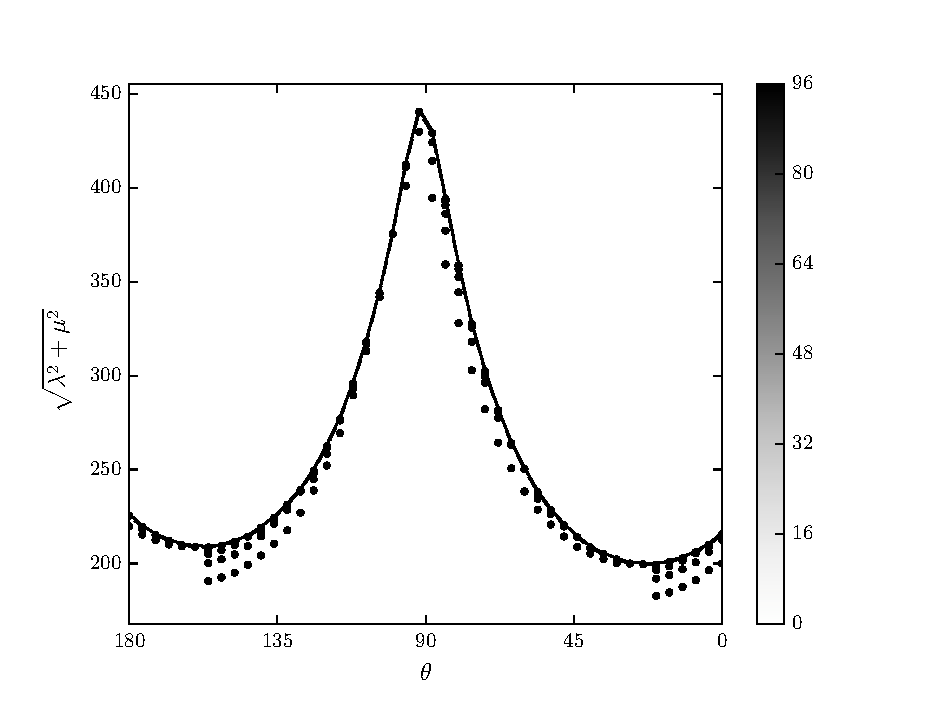
\includegraphics{./fig/ch3/pull/b100/grid.eps}
      \end{center}      
      \caption{Plot of the minimum critical magnitude for detachment as in Figure~\ref{fig:pull:ref}. The torsional spring strength is increased, $\beta=100$.
      \label{fig:pull:b100}}
   \end{figure}

For the compression experiment $\beta$ was already sufficiently large for a fiber to stand freely. In the case of the detachment experiment $\beta=1$ is a magnitude lower and the fiber will not be able to stand freely. Like before, we focus only on increasing $\beta$.

With increased $\beta$ the story does not signficantly change. Figure~\ref{fig:pull:b10} and Figure~\ref{fig:pull:b100} show plots that are similar in general shape to the reference parameters. When the dynamics of a detachment are observed they are also very similar to the reference parameters. However, the values of extrema are different with larger $\beta$. The local minimum of the critical detachment load to the left of the maximum value is larger as $\beta$ increases. In contrast, the minimum value to the right of the maximum value of smaller as $\beta$ increases. This means the asymmetry in the plot is more exaggerated with larger $\beta$. This observation is consistent with the given explanation for the asymmetry being related to torsional springs near the root particle of the fiber. Lastly, the maximum critical magnitude decreases as $\beta$ increases.

   \begin{figure}[t]
      \begin{center}
         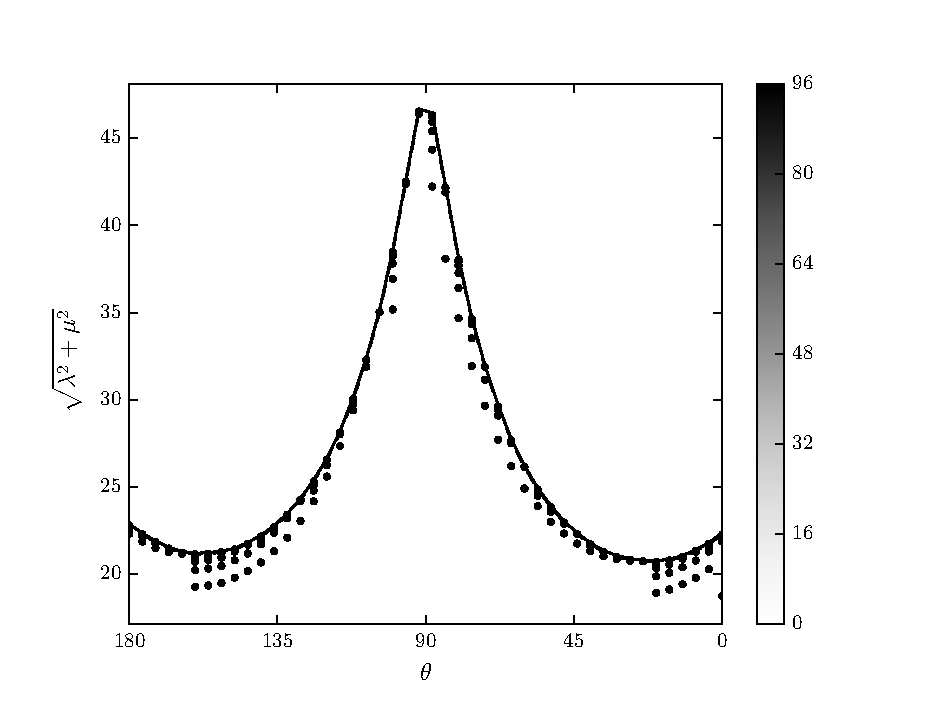
\includegraphics{./fig/ch3/pull/eb0.1_et0.1/grid.eps}
      \end{center}      
      \caption{Plot of the minimum critical magnitude for detachment as in Figure~\ref{fig:pull:ref}. The strength of the vdW interaction for the bottom and top substrate are decreased, $\eps_-=0.1$ and $\eps_+=0.1$.
      \label{fig:pull:eb0.1_et0.1}}
   \end{figure}
   
   \begin{figure}[t]
      \begin{center}
         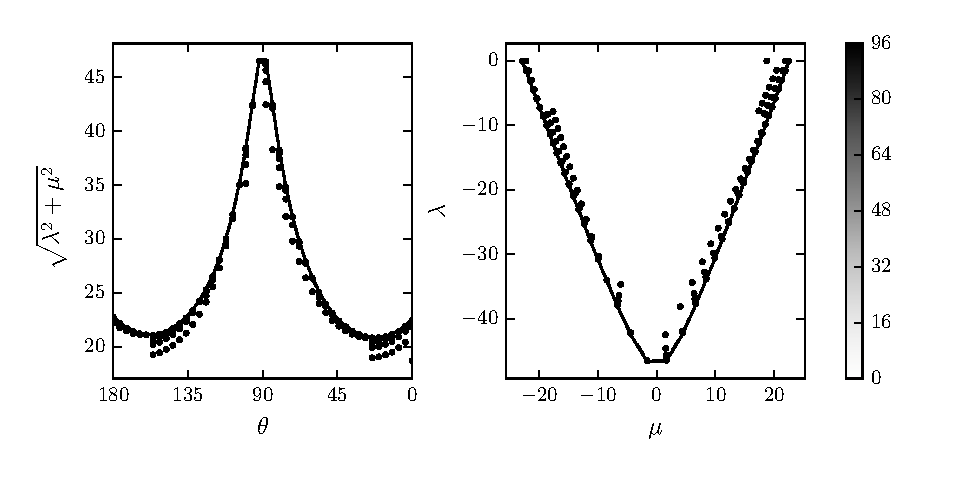
\includegraphics{./fig/ch3/pull/eb0.1_et0.1_e0.1/grid.eps}
      \end{center}      
      \caption{Plot of the minimum critical magnitude for detachment as in Figure~\ref{fig:pull:ref}. The strength of the vdW interaction for all particles are decreased, $\eps_-=0.1$, $\eps_+=0.1$, and $\eps=0.1$.
      \label{fig:pull:eb0.1_et0.1_e0.1}}
   \end{figure}

   \begin{figure}[t]
      \begin{center}
         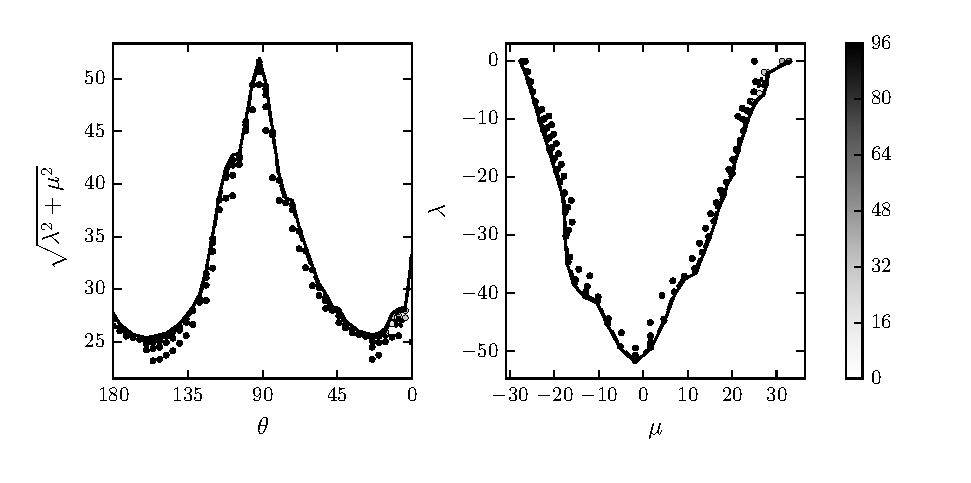
\includegraphics{./fig/ch3/pull/eb0.1/grid.eps}
      \end{center}      
      \caption{Plot of the minimum critical magnitude for detachment as in Figure~\ref{fig:pull:ref}. The strength of the vdW interaction for the bottom substrate is decreased, $\eps_-=0.1$. In both plots there is a black star marker which corresponds to a detachment magnitude that happens below what we consider the critical magnitude.
      \label{fig:pull:eb0.1}}
   \end{figure}

   \begin{figure*}[t]
      \centering
      \begin{subfigure}{.5\textwidth}
         \centering
         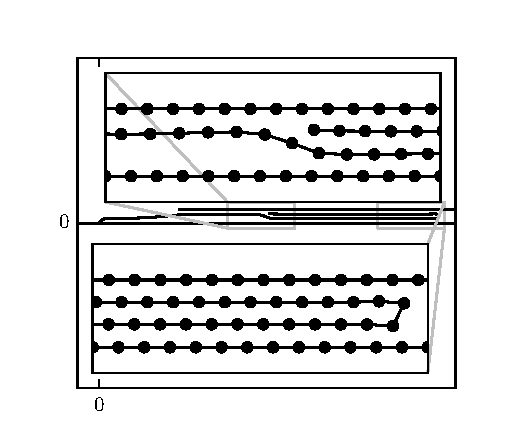
\includegraphics{./fig/ch3/pull/eb0.1/l0_m32.8.eps}
         \caption{$\lambda=0$ and $\mu=32.8$. \label{subfig:folded_over}}
      \end{subfigure}%
      ~
      \begin{subfigure}{.5\textwidth}
         \centering
         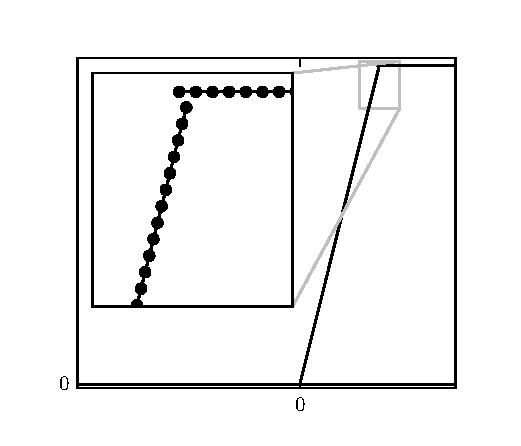
\includegraphics{./fig/ch3/pull/eb0/t76_m4.eps}
         \caption{$\lambda\approx3.88$ and $\mu\approx0.968$\label{subfig:barely_adhered}}
      \end{subfigure}
      \caption{Configuration (a) is an archetypal example of angles of loads on the top substrate that are close to 0. Such loads will often fold ontop of themselves as the top substrate pulls them to the right. Configuration (b) is an archetypal example of the white simulations in the plot for Figure~\ref{fig:pull:eb0}. The reference parameters are modified differently in both examples, for (a) $\eps_-=0.1$ and for (b) $\eps_-=0$.\label{fig:pull_equil}} 
   \end{figure*}

   \begin{figure*}[t]
      \centering
      \begin{subfigure}{.5\textwidth}
         \centering
         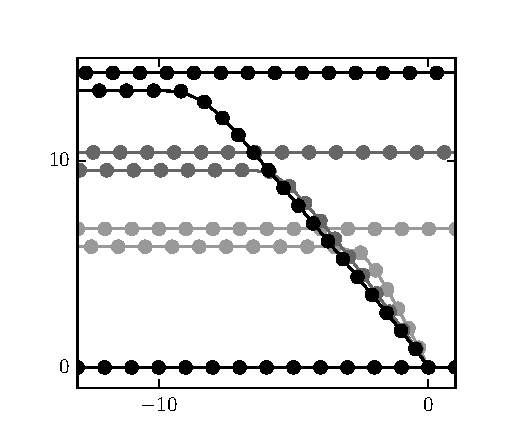
\includegraphics{./fig/ch3/pull/unzip_anim.eps}
         \caption{\label{subfig:unzip}}
      \end{subfigure}%
      ~
      \begin{subfigure}{.5\textwidth}
         \centering
         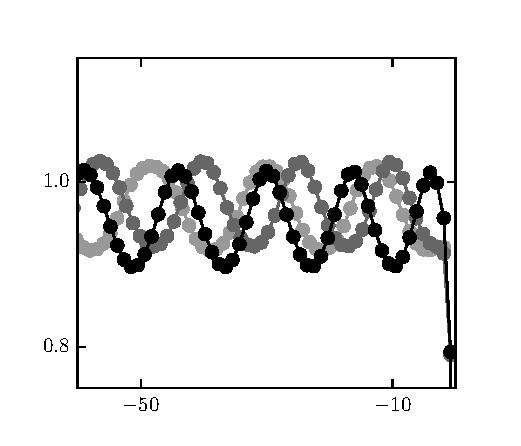
\includegraphics{./fig/ch3/pull/wave_anim.eps}
         \caption{\label{subfig:travel_waves}}
      \end{subfigure}
      \caption{Three time steps of a moving fiber as examples for the kinds of detachemnt modes. Darker fibers are later in the evolution of time. For (a) we see an unzipping mode of detachment were a the top substrate and fiber break the vdW interaction between one particle at a time. For (b) wee see a propogation of waves through a fiber.\label{fig:animation}}  
   \end{figure*}

   \begin{figure}[t]
      \begin{center}
         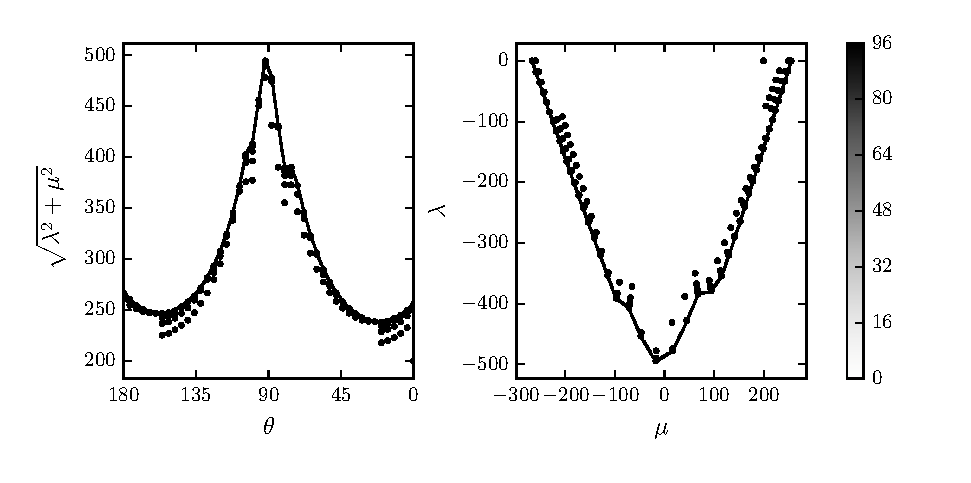
\includegraphics{./fig/ch3/pull/et10/grid.eps}
      \end{center}      
      \caption{Plot of the minimum critical magnitude for detachment as in Figure~\ref{fig:pull:ref}. The strength of the vdW interaction for the top substrate is increased, $\eps_+=10$.
      \label{fig:pull:et10}}
   \end{figure}

   \begin{figure}[t]
      \begin{center}
         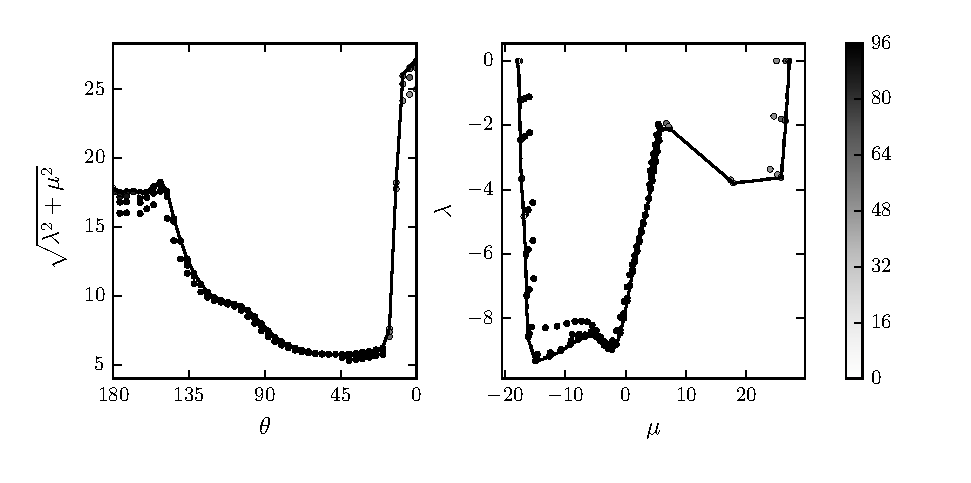
\includegraphics{./fig/ch3/pull/eb0.01/grid.eps}
      \end{center}      
      \caption{Plot of the minimum critical magnitude for detachment as in Figure~\ref{fig:pull:ref}. The strength of the vdW interaction for the bottom substrate is decreased, $\eps_-=0.01$. 
      \label{fig:pull:eb0.01}}
   \end{figure}
   
   \begin{figure}[t]
      \begin{center}
         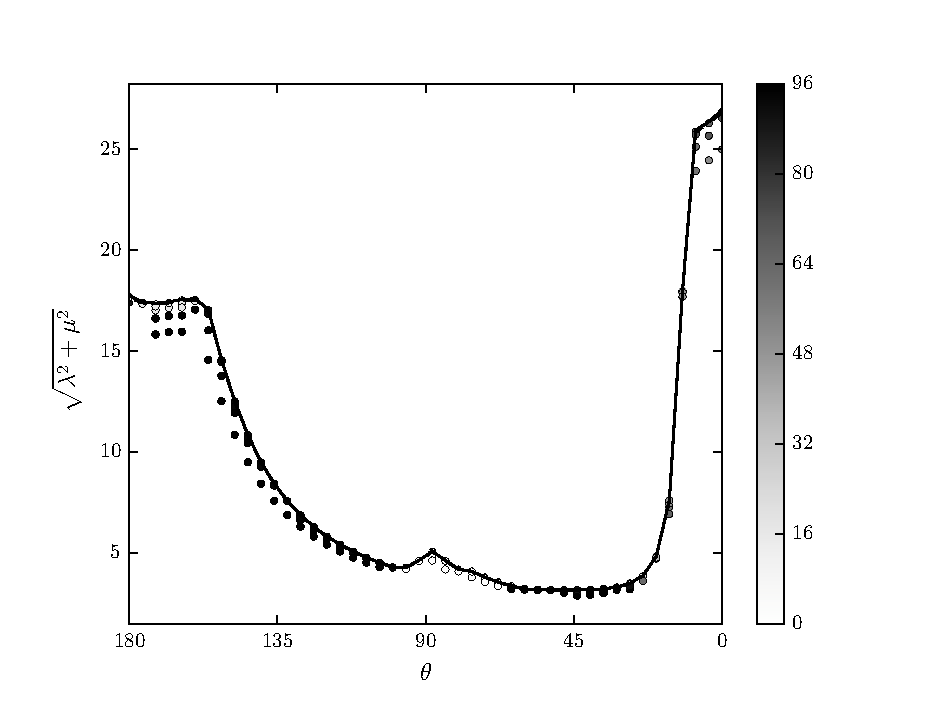
\includegraphics{./fig/ch3/pull/eb0/grid.eps}
      \end{center}      
      \caption{Plot of the minimum critical magnitude for detachment as in Figure~\ref{fig:pull:ref}. The strength of the vdW interaction for the bottom substrate is removed, $\eps_-=0$. Note that simulation circles that are white are not the same as star markers representing isolated detachments.
      \label{fig:pull:eb0}}
   \end{figure}

\subsection{Varying $\eps^-$, $\eps^+$, and $\eps$} \label{section:detachment:eps}

Varying vdW interaction strengths has the most significant effect on the results of the detachment experiment that we have observed. First, we consider decreasing $\eps_-$ and $\eps_+$ to $0.1$ and then all three vdW interactions, $\eps_- = \eps_+ = \eps = 0.1$. Second, we consider the case were only $\eps_-=0.1$ and the case where only $\eps_+=10$. Lastly, we consider decreasing $\eps_-$ further, exploring both $\eps_-=0.01$ and $\eps_-=0$.

For $\eps_- = \eps_+ = 0.1$ the critical magnitude for detachment is decreased for all angles of the load by approximately an order of magnitude relative to the critical magnitude of the reference parameters. Figure~\ref{fig:push:eb0.1_et0.1} demonstrates the linear relationship between the critical detachment load and the decrease in the substrate vdW interaction strengths. The modes of detachment are also the same. For $\theta$ sufficiently larger or smaller than $90$\textdegree\ the top substrate detaches in the sliding mode, and in the brute force mode otherwise. The asymmetry of minimums of the plot is increased. The minimum value of the critical magnitude on the right is smaller than the reference parameters, and the  value on the left is larger, increasing the gap between the values. If we modify the fiber vdW interaction strength so that all values are equal, that is $\eps_- = \eps_+ = \eps = 0.1$ then the minimum values of the plot are less asymmetric (the gap is decreased). Figure~\ref{fig:pull:eb0.1_et0.1_e0.1} shows the critical detachment magnitude for these equal values. The observations we made for the prior plot (Figure~\ref{fig:pull:eb0.1_et0.1}) hold here as well. That is, all values of the critical detachment magnitude are approximately an order of magnitude lower than the reference case, and the modes of detachment are similar.

Consider instead that we decrease $\eps_-$ only, i.e. $\eps_-=0,1$. The plot of the critical detachment magnitude in Figure~\ref{fig:pull:eb0.1} is a comparably similar shape to the reference parameters but there is plateau on either side of $\theta=90$\textdegree. Also, for $\theta$ near $0$\textdegree\ there is an interesting change in the method of detachment for the top substrate. In fact, the modes of detachment are different for any $\theta$. For $\theta$ not near the maximum value of the critical detachment magnitude there is a new mode of detachment consisting of propagating waves. The substrate can still be considered as sliding and it may be that the mechanics of sliding for the reference parameters are precisely the same as what gives propagating waves for this modification of parameters. Likewise, for $\theta$ near $90$\textdegree\ the dynamics of detachment are not brute force but an ``unzipping'' of the fiber. Figure~\ref{subfig:travel_waves} shows the propagating waves at three distinct time steps, darker greys are later in time. Note that the waves do not travel through the fiber at a uniform speed necessarily. Figure~\ref{subfig:unzip} shows the ``unzipping'' of a fiber at three distinct time steps, colored in the same way. A fiber is said to ``unzip'' from a substrate if one particle breaks adhesion with the substrate at a time and in contiguous sequence from the initially detached particle. These two modes of detachment, unzipping and wave propagated sliding, seem to be the analogues of brute force and ``simple'' sliding we saw before. Not only are the previous two modes of detachment arguably special cases of these modes, the values of $\theta$ for which they occur are similar.

Values of $\theta$ near $0$\textdegree\ are interesting in there own right. Every simulation below the critical detachment magnitude up until this point has maintained the flattened configuration and held true to our assumption that there is in fact a critical detachment magnitude of the load. This fails to be the case for small values of $\theta$ when $\eps_-=0.1$. There is one star simulation marker in the plot of Figure~\ref{fig:pull:eb0.01} that represents what we call an \textit{island detachment magnitude}. For many simulation points in the same region of the plot the adhesion of the fiber is also noticeable less than any other simulation, this is because this is the only time the fiber has folded up and onto itself during the dynamics of detachment. Figure~\ref{subfig:folded_over} shows the equilibrium configuration for a load on the top substrate that is not an island detachment magnitude. An explanation for this behavior is that if the amplitude and frequency of the propagating waves is just right the particles on the fiber will start to crystallize stiffing the fiber and ultimately pulling it over onto itself as the detachment mode temporarily degenerates to simple sliding. The cause of isolated detachment magnitudes is then a complicated issue of whether or not the fiber particles crystallize with the particles on the top substrate in such a way to stay adhered or if the substrate has moved laterally a sufficient amount already to avoid re-adhering particles. Re-adhering particles are fiber particles shown near the root particle in Figure~\ref{subfig:folded_over}.

We attempt to avoid the issue of isolated detachment magnitudes by performing an additional simulation with a magnitude slightly larger for any simulation where the top substrate detaches from the fiber. Even if there are isolated detachment magnitudes there is still good reason to believe that there is a boundary between magnitudes of the load that cause the top substrate to strictly detach regardless of how large the values are. In an attempt to avoid island detachment magnitudes and find this boundary in all cases we believe the additional simulation is a satisfactory heuristic.

Increasing $\eps_+$ by an order of magnitude from the reference parameters alone has comparable effects to decreasing $\eps_-$. The two modes of detachment previously described are still present, namely that of unzipping and wave propagated sliding. However, those detachment modes can also be mixed. For some values of $\theta$ near $0$\textdegree\ the mode of detachment is still sliding and the plateau in $\theta$ is still related to a notion of a critical $\theta$ where the mode of detachment shifts (in this case from mixed to strictly unzipping), but in between these modes there is a mixture of both. First, the detachment mode will be wave propagated sliding and then after sufficiently many waves have been generated the mode will switch to unzipping. We conjecture that waves are generated with higher amplitude and frequency and so when enough waves are present in the fiber the top substrate is only adhered to a fraction of fiber particles and can then change modes of detachment to unzipping. Note also that the behavior of the dynamics near $\theta=0$ is more similar to the reference plot (see Figure~\ref{fig:pull:ref}) than the plot of $\eps_-=0.1$.

Lastly, we decrease $\eps_-$ to values $0.01$ and $0$. The plot of the critical magnitude has been relatively comparable for all values that we've seen so far with only minor disparities. When we decrease $\eps_-$ even further than we did previously the picture changes significantly. In Figure~\ref{fig:pull:eb0.01} the values of the critical magnitude are much smaller than the reference parameter values and still smaller than the critical magnitude values of $\eps_-=0.1$. For $\theta$ near $0$\textdegree\ the same dynamics of the fiber folding over occurs. There are likely island detachment magnitudes below the critical magnitude line even though none are shown in the plot. The primary mode of detachment is unzipping. Sliding only appears to occur for values of $\theta$ near either $0$\textdegree\ or $180$\textdegree. The asymmetry in the plot must be caused by the direction the fiber is flattened although the exact relationship between the two is not understood. When $\eps_-$ is decreased to the point of vanishing, i.e. $\eps_-=0$, we have a similar plot as shown in Figure~\ref{fig:pull:eb0}. The notable differences are values near $\theta=0$ which give an equilibrium configuration shown in Figure~\ref{subfig:barely_adhered}. It is clear that the magnitude of the load on the top substrate is not strong enough to break a single adhesive bond between the top substrate and a fiber particle. Thus, the configuration is in large part caused by the torsional spring strength. An important detail is that the detachment mode of unzipping is a consorted effort between the vdW interaction strengths, the torsional spring strength, and the magnitude of the load on the top substrate.

\subsection{Varying $\gamma$}

   \begin{figure}[t]
      \begin{center}
         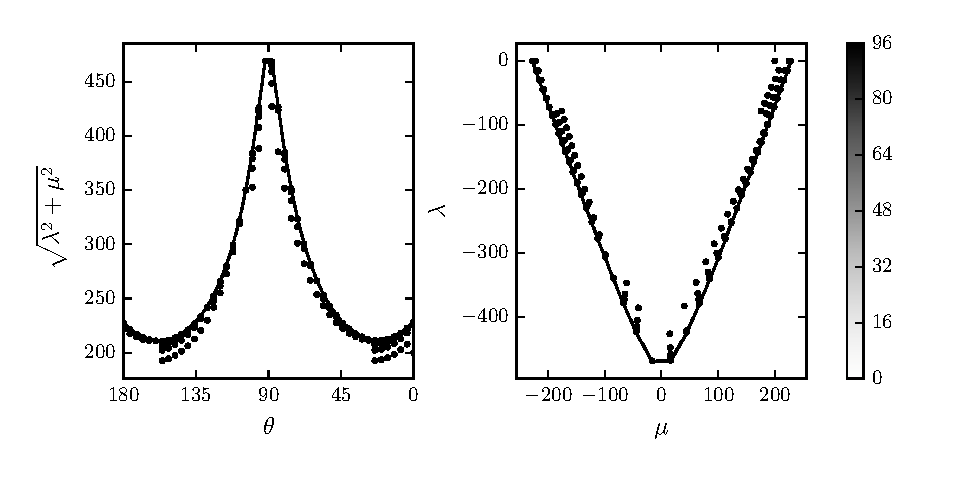
\includegraphics{./fig/ch3/pull/g1000/grid.eps}
      \end{center}      
      \caption{Plot of the minimum critical magnitude for detachment as in Figure~\ref{fig:pull:ref}. The extensible spring constant is increased, $\gamma=1000$.
      \label{fig:pull:g1000}}
   \end{figure}

We modify the extensible spring constant to ensure the reference selection, $\gamma=100$, is sufficiently stiff. Although larger values of $\gamma$ will alter the dynamics and equilibrium configurations we want extensible springs to be able to relax without significant changes between results with our selected value and larger values. Figure~\ref{fig:pull:g1000} shows the plot of the critical magnitude of the load. The similarity between this plot and the reference plot in Figure~\ref{fig:pull:ref} suggests our selection of $\gamma$ is sufficient.


\subsection{Bottom substrate with uniform potential} \label{section:detachment:pressure}

   \begin{figure}[t!]
      \begin{center}
         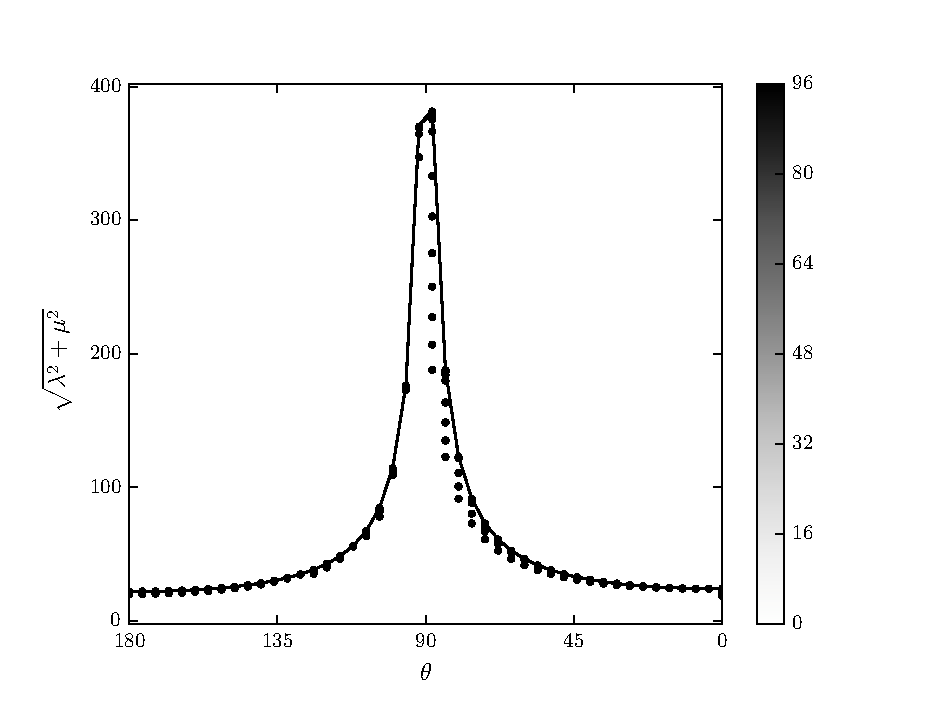
\includegraphics{./fig/ch3/pull/p1/grid.eps}
      \end{center}      
      \caption{Plot of the minimum critical magnitude for detachment as in Figure~\ref{fig:pull:ref}. The bottom substrate is replaced with a continuum of particles, that is the vdW interaction is integrated over the entire real line. The strength of the continuum vdW interaction is $p=1$.
      \label{fig:pull:p1}}
   \end{figure}
   
   \begin{figure}[th!]
      \begin{center}
         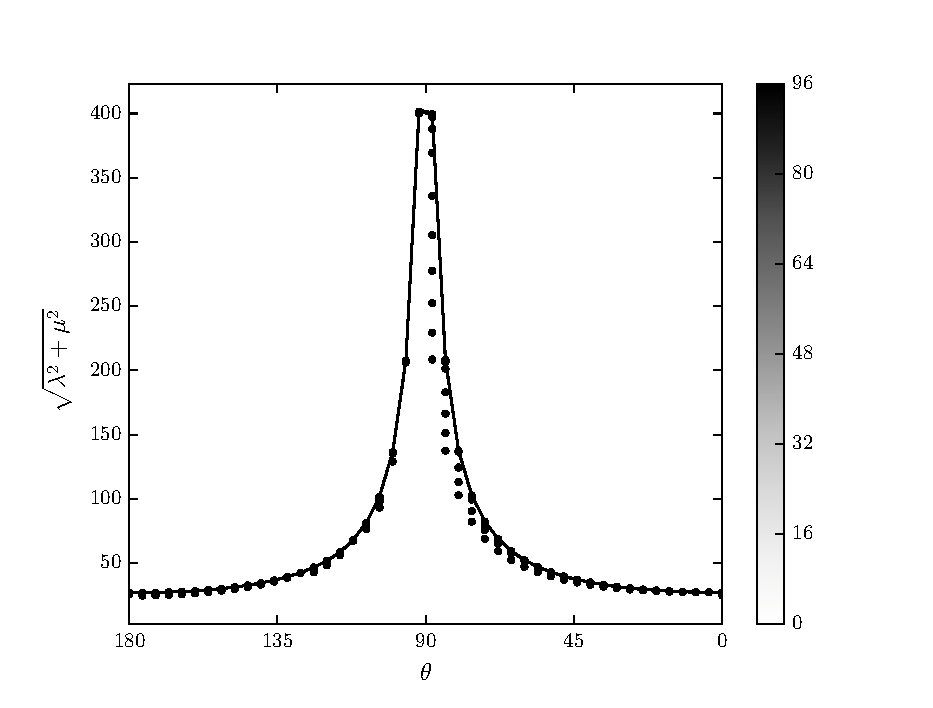
\includegraphics{./fig/ch3/pull/p10/grid.eps}
      \end{center}      
      \caption{Plot of the minimum critical magnitude for detachment as in Figure~\ref{fig:pull:ref}. The bottom substrate is replaced with a continuum of particles. The strength of the continuum vdW interaction is $p=10$.
      \label{fig:pull:p10}}
   \end{figure}

In section~\ref{section:compression:pressure} we replaced the bottom substrate particle-particle potential with a uniform potential. We make the same modification here and briefly discuss the effects on the model under the detachment experiment.

Figure~\ref{fig:pull:p1} and Figure~\ref{fig:pull:p10} show the critical magnitude of the load with the modified bottom substrate potential. The dynamics of the detachment situation are the same as the reference parameters, i.e. that there are two detachment modes: sliding and brute force. There is still a maximum of the critical load near $\theta=90$\textdegree\ and still likely a critical angle were the detachment mode changes. However, the minimums on either side of the plot have changed. An explanation is that there is no resistance for the fiber particles to prevent horizontal displacement because the potential is uniform. Any vertical component of the load does not assist the top substrate in detaching from the fiber which means the minimums on the left and right of the plot should be at $\theta=0$ and $\theta=180$.

\section{Conclusion}

Three separate experiments for the model were explored to discover trends in equilibrium configurations. An adhesive heuristic was used in all experiments successfully to categorize equilibrium configurations qualitatively. For the free standing experiment a linear relationship was observed between $\eps_-$ and $\beta$ describing the change from a slanting to flattened configuration. Another linear relationship between flattened and crystallizing configurations was also observed. The compression experiment also gave proportional relationships between $\lambda$ and $\mu$ for many of the explored variations of parameters. Large values of $\beta$ and smaller values of $\eps_+$ gave significantly different results from the reference parameters. The detachment experiment demonstrated different dynamics of detachment (sliding and unzipping) and that a critical magnitude for detachment existed with some explainable exceptions. It also showed two local minimums for the critical magnitude and one maximum as a function of $\theta$ for the reference parameters and variations of the reference parameters.
